% STS2 DESIGN VISUALS V2
% Reviewed target architecture, generated for technical review.
% Compile: pdflatex STS2_DESIGN_VISUALS_V2.tex (twice)
\documentclass[10pt]{article}
\usepackage[a4paper,landscape,margin=10mm]{geometry}
\usepackage[T1]{fontenc}
\usepackage[sc]{mathpazo}
\usepackage{microtype}
\usepackage{tikz}
\usetikzlibrary{arrows.meta,positioning,fit,calc,backgrounds,shapes.geometric,shapes.multipart,decorations.pathreplacing,matrix}
\usepackage{xcolor}
\usepackage{adjustbox}
\usepackage{hyperref}
\hypersetup{hidelinks}
\pagestyle{empty}
\setlength{\parindent}{0pt}

\definecolor{runtime}{HTML}{EAF0FF}
\definecolor{core}{HTML}{EAF8EC}
\definecolor{journal}{HTML}{FFF0EE}
\definecolor{observer}{HTML}{F6EDFA}
\definecolor{edge}{HTML}{FFF5E6}
\definecolor{external}{HTML}{F4F4F4}
\definecolor{risk}{HTML}{FFE3E3}
\definecolor{good}{HTML}{E2F5E7}
\definecolor{policy}{HTML}{E8F7F5}
\definecolor{ink}{HTML}{263238}
\definecolor{muted}{HTML}{607D8B}
\definecolor{blue}{HTML}{3F6FB5}
\definecolor{red}{HTML}{B54A4A}
\definecolor{purple}{HTML}{7A4E9B}
\definecolor{orange}{HTML}{B56A24}
\definecolor{green}{HTML}{39784A}

\tikzset{
  >=Latex,
  every node/.style={font=\small,text=ink},
  box/.style={draw=ink!65,rounded corners=2.5pt,fill=runtime,minimum height=11mm,minimum width=35mm,align=center,inner sep=4pt},
  corebox/.style={box,fill=core},
  journalbox/.style={box,fill=journal,draw=red!75},
  obsbox/.style={box,fill=observer,draw=purple!70},
  edgebox/.style={box,fill=edge,draw=orange!75},
  extbox/.style={box,fill=external,dashed},
  policybox/.style={box,fill=policy,draw=green!70},
  riskbox/.style={box,fill=risk,draw=red!80},
  goodbox/.style={box,fill=good,draw=green!75},
  tinybox/.style={draw=ink!60,rounded corners=2pt,fill=white,align=center,inner sep=3pt,font=\footnotesize},
  state/.style={draw=ink!65,rounded corners=6pt,fill=runtime,minimum width=29mm,minimum height=10mm,align=center},
  term/.style={state,fill=good},
  arrow/.style={->,very thick,draw=ink!75},
  async/.style={->,thick,dashed,draw=purple},
  write/.style={->,very thick,draw=red},
  effect/.style={->,very thick,draw=orange},
  policyarr/.style={->,very thick,draw=green},
  fail/.style={->,very thick,dashed,draw=red},
  note/.style={draw=ink!30,rounded corners=2pt,fill=white,align=left,inner sep=5pt,font=\footnotesize,text width=70mm},
  pill/.style={draw=ink!45,rounded corners=7pt,fill=white,inner xsep=6pt,inner ysep=2pt,font=\footnotesize\bfseries},
  label/.style={font=\footnotesize,align=center,fill=white,inner sep=1.5pt},
}
\newcommand{\code}[1]{\texttt{#1}}
\newcommand{\pagehead}[2]{%
  \begin{minipage}[t]{0.73\linewidth}
    {\Large\bfseries #1}\\[-1mm]
    {\small\color{muted}#2}
  \end{minipage}\hfill
  \begin{minipage}[t]{0.25\linewidth}\raggedleft
    {\footnotesize STS2 reviewed target design}\\
    {\scriptsize branch snapshot c9fbd1e40ec8}
  \end{minipage}
  \vspace{3mm}\hrule\vspace{4mm}
}
\newcommand{\legend}{%
\tikz[baseline=-0.7ex]\node[box,minimum width=7mm,minimum height=4mm,inner sep=1pt]{}; runtime\quad
\tikz[baseline=-0.7ex]\node[corebox,minimum width=7mm,minimum height=4mm,inner sep=1pt]{}; pure Core\quad
\tikz[baseline=-0.7ex]\node[journalbox,minimum width=7mm,minimum height=4mm,inner sep=1pt]{}; journal\quad
\tikz[baseline=-0.7ex]\node[edgebox,minimum width=7mm,minimum height=4mm,inner sep=1pt]{}; effect edge\quad
\tikz[baseline=-0.7ex]\node[obsbox,minimum width=7mm,minimum height=4mm,inner sep=1pt]{}; observer\quad
\tikz[baseline=-0.7ex]\node[policybox,minimum width=7mm,minimum height=4mm,inner sep=1pt]{}; policy/security
}

\begin{document}

% -----------------------------------------------------------------------------
% Cover
\begin{center}
\vspace*{13mm}
{\fontsize{30}{34}\selectfont\bfseries STS2 Design Visuals v2}\\[3mm]
{\Large Reviewed target architecture for a SQL Tools Service that explains itself while it runs}\\[10mm]
\begin{adjustbox}{max width=0.98\linewidth,max totalheight=0.78\textheight,center}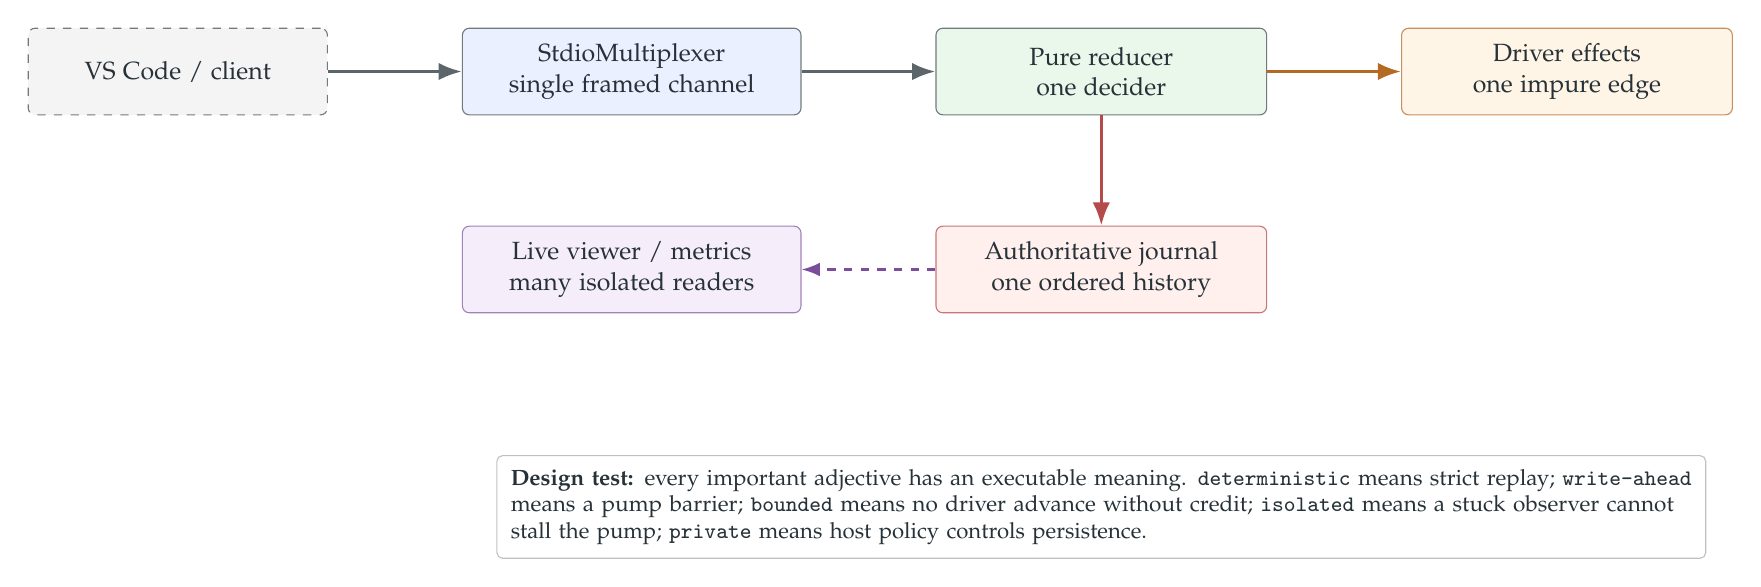
\begin{tikzpicture}[node distance=14mm and 17mm]
  \node[extbox,minimum width=38mm] (client) {VS Code / client};
  \node[box,right=of client,minimum width=43mm] (mux) {StdioMultiplexer\\single framed channel};
  \node[corebox,right=of mux,minimum width=42mm] (core) {Pure reducer\\one decider};
  \node[journalbox,below=of core,minimum width=42mm] (jr) {Authoritative journal\\one ordered history};
  \node[edgebox,right=of core,minimum width=42mm] (driver) {Driver effects\\one impure edge};
  \node[obsbox,below=of mux,minimum width=43mm] (view) {Live viewer / metrics\\many isolated readers};
  \draw[arrow] (client) -- (mux);
  \draw[arrow] (mux) -- (core);
  \draw[write] (core) -- (jr);
  \draw[effect] (core) -- (driver);
  \draw[async] (jr) -- (view);
  \node[note,below=18mm of jr,text width=150mm] {
    \textbf{Design test:} every important adjective has an executable meaning.
    \code{deterministic} means strict replay; \code{write-ahead} means a pump barrier;
    \code{bounded} means no driver advance without credit; \code{isolated} means a stuck
    observer cannot stall the pump; \code{private} means host policy controls persistence.
  };
\end{tikzpicture}\end{adjustbox}\\[11mm]
{\small \legend}\\[12mm]
{\footnotesize Companion files: \code{01\_TECHNICAL\_REVIEW.md}, \code{03\_TARGET\_DESIGN.md}, and \code{05\_NEXT\_STEPS.md}.}
\end{center}
\clearpage

% -----------------------------------------------------------------------------
\pagehead{1. System context and trust boundaries}{One process and one stdio channel, with explicit persistence and privacy boundaries.}
\begin{adjustbox}{max width=0.98\linewidth,max totalheight=0.78\textheight,center}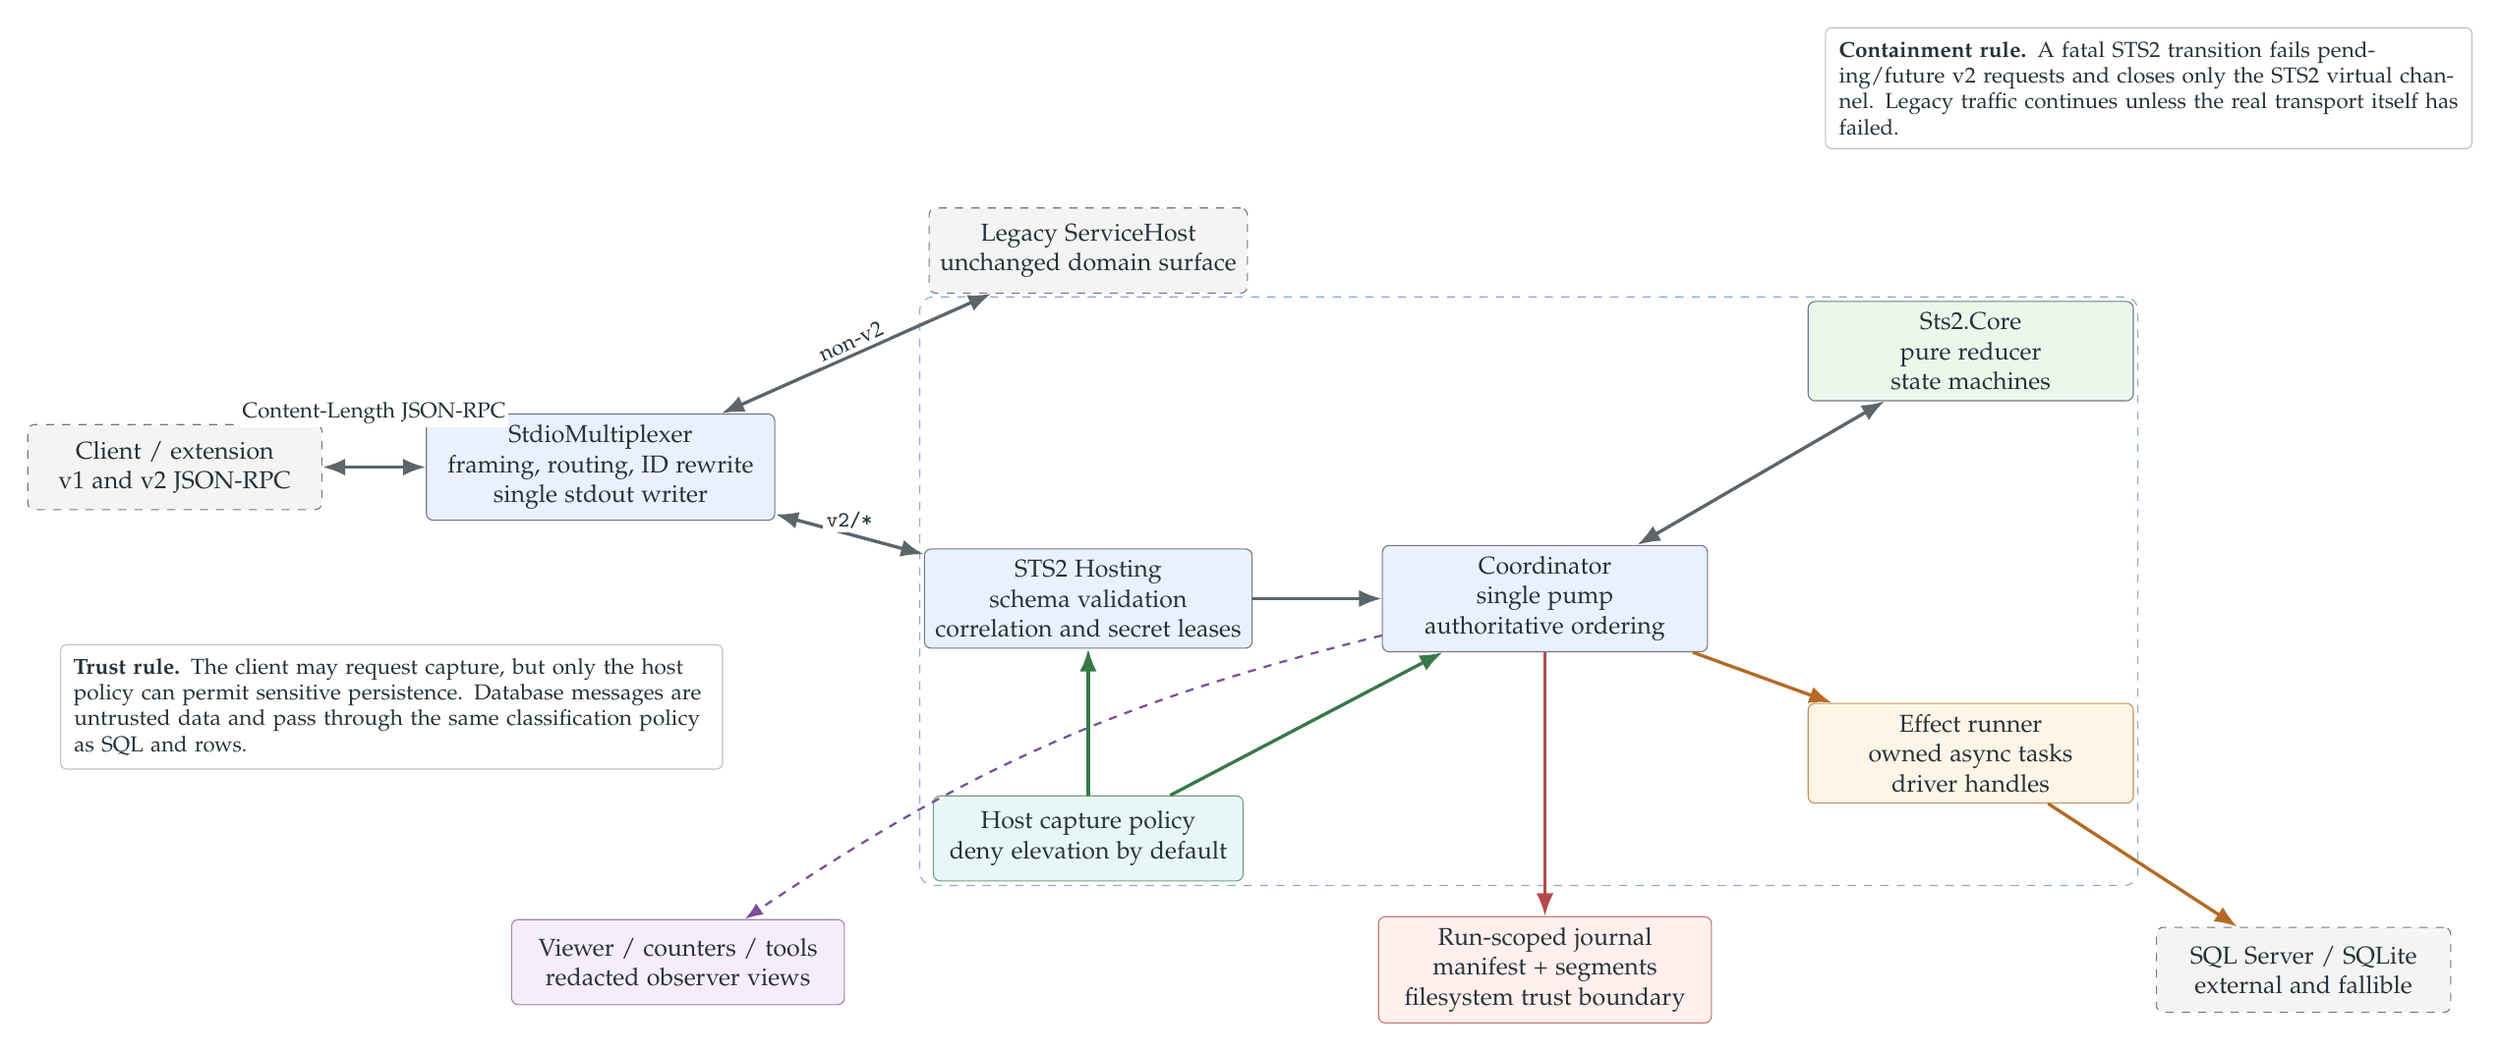
\begin{tikzpicture}[x=1cm,y=1cm]
  \node[extbox,minimum width=38mm] (client) at (1.5,7.7) {Client / extension\\v1 and v2 JSON-RPC};
  \node[box,minimum width=45mm] (mux) at (7.0,7.7) {StdioMultiplexer\\framing, routing, ID rewrite\\single stdout writer};
  \node[extbox,minimum width=40mm] (legacy) at (13.3,10.5) {Legacy ServiceHost\\unchanged domain surface};
  \node[box,minimum width=40mm] (host) at (13.3,6.0) {STS2 Hosting\\schema validation\\correlation and secret leases};
  \node[box,minimum width=42mm] (coord) at (19.2,6.0) {Coordinator\\single pump\\authoritative ordering};
  \node[corebox,minimum width=42mm] (core) at (24.7,9.2) {Sts2.Core\\pure reducer\\state machines};
  \node[edgebox,minimum width=42mm] (runner) at (24.7,4.0) {Effect runner\\owned async tasks\\driver handles};
  \node[extbox,minimum width=38mm] (db) at (29.0,1.2) {SQL Server / SQLite\\external and fallible};
  \node[journalbox,minimum width=43mm] (fs) at (19.2,1.2) {Run-scoped journal\\manifest + segments\\filesystem trust boundary};
  \node[obsbox,minimum width=43mm] (viewer) at (8.0,1.3) {Viewer / counters / tools\\redacted observer views};
  \node[policybox,minimum width=40mm] (policy) at (13.3,2.9) {Host capture policy\\deny elevation by default};
  \draw[arrow,<->] (client.east) -- node[label,above=5mm,fill=white,inner sep=1pt]{Content-Length JSON-RPC} (mux.west);
  \draw[arrow,<->] (mux) -- node[label,above,sloped]{non-v2} (legacy);
  \draw[arrow,<->] (mux) -- node[label,above]{\code{v2/*}} (host);
  \draw[arrow] (host) -- (coord);
  \draw[arrow,<->] (coord) -- (core);
  \draw[effect] (coord) -- (runner);
  \draw[effect] (runner) -- (db);
  \draw[write] (coord) -- (fs);
  \draw[async] (coord) to[bend right=10] (viewer);
  \draw[policyarr] (policy) -- (host);
  \draw[policyarr] (policy) -- (coord);
  \begin{scope}[on background layer]
    \node[draw=blue!60,dashed,rounded corners=5pt,fit=(host)(coord)(core)(runner)(policy),inner sep=5mm,
      label={[blue,font=\bfseries\footnotesize]above:STS2 session boundary}] {};
  \end{scope}
  \node[note,text width=82mm] at (4.3,4.6) {
    \textbf{Trust rule.} The client may request capture, but only the host policy can permit
    sensitive persistence. Database messages are untrusted data and pass through the same
    classification policy as SQL and rows.
  };
  \node[note,text width=80mm] at (27.0,12.6) {
    \textbf{Containment rule.} A fatal STS2 transition fails pending/future v2 requests and
    closes only the STS2 virtual channel. Legacy traffic continues unless the real transport
    itself has failed.
  };
\end{tikzpicture}\end{adjustbox}
\clearpage

% -----------------------------------------------------------------------------
\pagehead{2. Ownership and orderly shutdown}{A single ownership tree prevents orphan tasks, sessions, secrets, and observer workers.}
\begin{adjustbox}{max width=0.98\linewidth,max totalheight=0.78\textheight,center}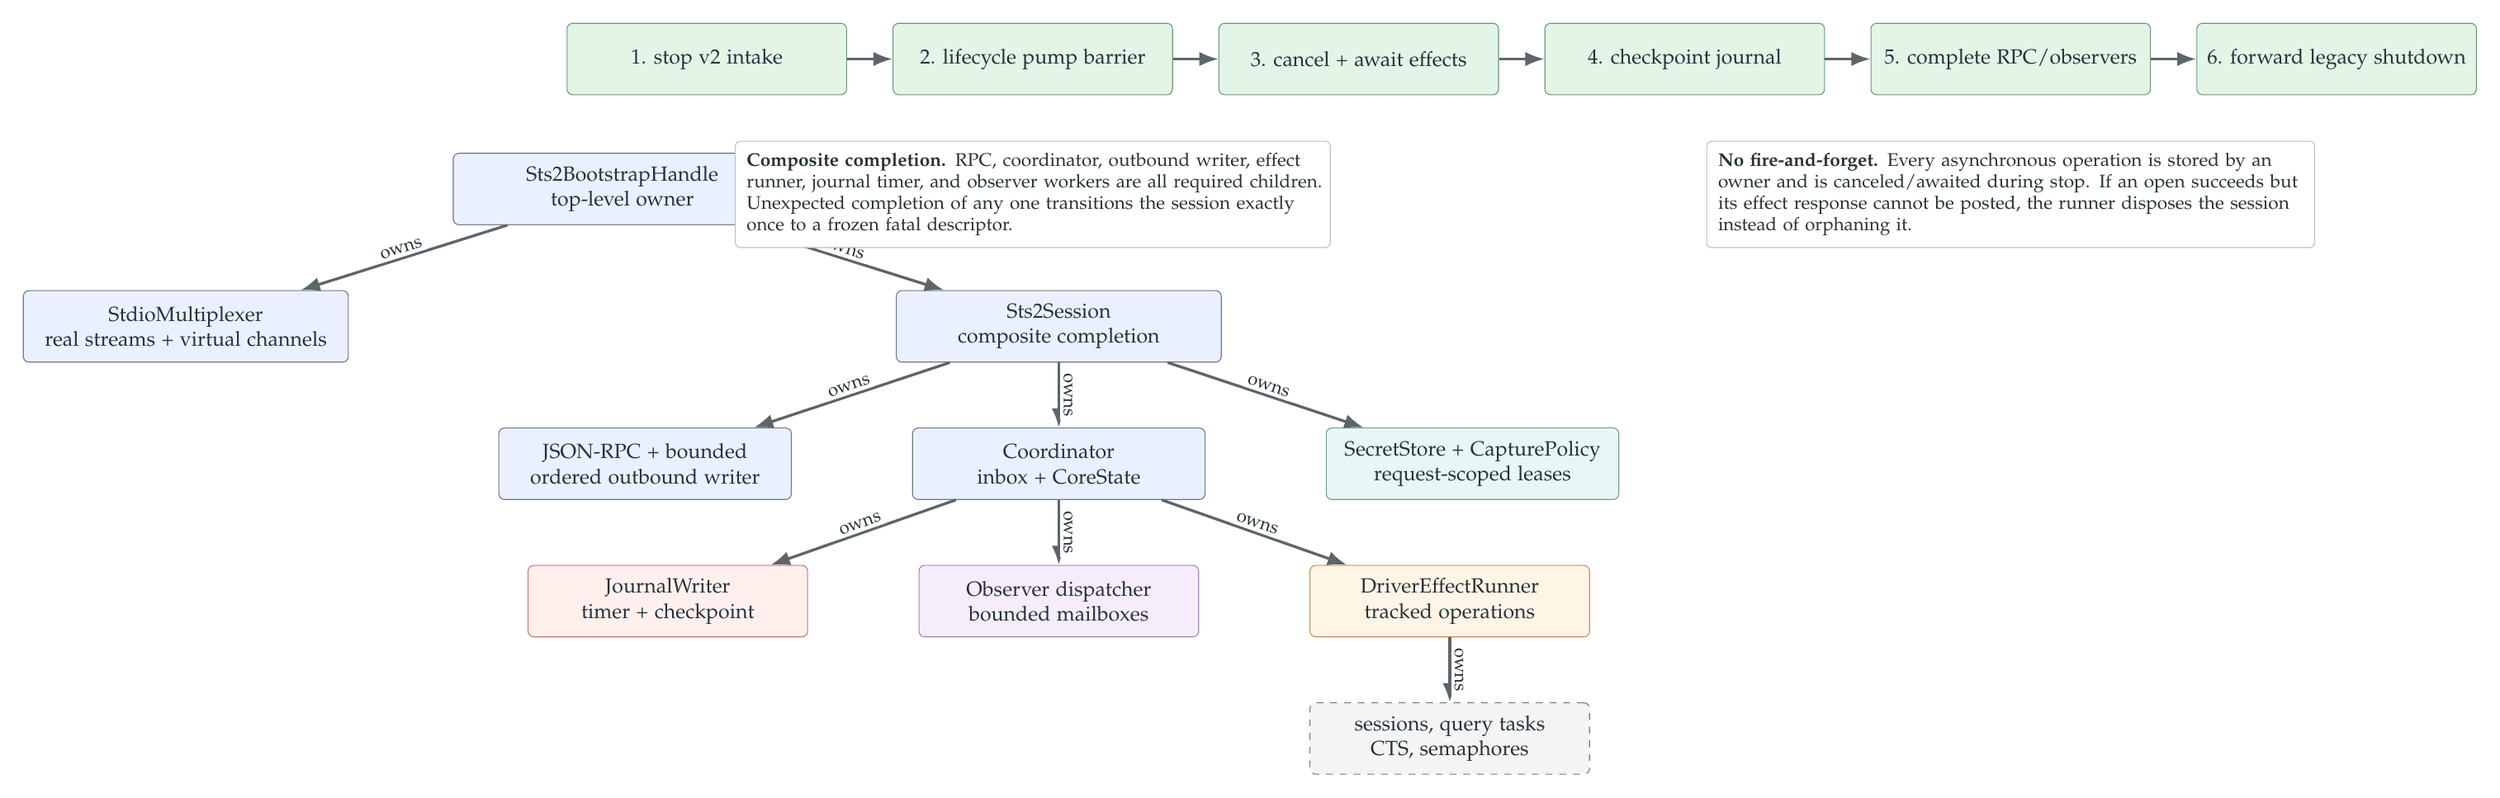
\begin{tikzpicture}[node distance=10mm and 16mm]
  \node[box,minimum width=52mm] (boot) {Sts2BootstrapHandle\\top-level owner};
  \node[box,below left=of boot,minimum width=50mm] (mux) {StdioMultiplexer\\real streams + virtual channels};
  \node[box,below right=of boot,minimum width=50mm] (session) {Sts2Session\\composite completion};
  \node[box,below left=of session,minimum width=45mm] (rpc) {JSON-RPC + bounded\\ordered outbound writer};
  \node[box,below=of session,minimum width=45mm] (coord) {Coordinator\\inbox + CoreState};
  \node[policybox,below right=of session,minimum width=45mm] (secret) {SecretStore + CapturePolicy\\request-scoped leases};
  \node[journalbox,below left=of coord,minimum width=43mm] (journal) {JournalWriter\\timer + checkpoint};
  \node[obsbox,below=of coord,minimum width=43mm] (obs) {Observer dispatcher\\bounded mailboxes};
  \node[edgebox,below right=of coord,minimum width=43mm] (effects) {DriverEffectRunner\\tracked operations};
  \node[extbox,below=of effects,minimum width=43mm] (handles) {sessions, query tasks\\CTS, semaphores};
  \foreach \a/\b in {boot/mux,boot/session,session/rpc,session/coord,session/secret,coord/journal,coord/obs,coord/effects,effects/handles}
    \draw[arrow] (\a) -- node[label,sloped,above]{owns} (\b);

  \node[goodbox,minimum width=43mm] (s1) at (1.3,2.0) {1. stop v2 intake};
  \node[goodbox,minimum width=43mm,right=7mm of s1] (s2) {2. lifecycle pump barrier};
  \node[goodbox,minimum width=43mm,right=7mm of s2] (s3) {3. cancel + await effects};
  \node[goodbox,minimum width=43mm,right=7mm of s3] (s4) {4. checkpoint journal};
  \node[goodbox,minimum width=43mm,right=7mm of s4] (s5) {5. complete RPC/observers};
  \node[goodbox,minimum width=43mm,right=7mm of s5] (s6) {6. forward legacy shutdown};
  \draw[arrow] (s1) -- (s2); \draw[arrow] (s2) -- (s3); \draw[arrow] (s3) -- (s4);
  \draw[arrow] (s4) -- (s5); \draw[arrow] (s5) -- (s6);

  \node[note,text width=88mm,below=7mm of s2] {
    \textbf{Composite completion.} RPC, coordinator, outbound writer, effect runner, journal
    timer, and observer workers are all required children. Unexpected completion of any one
    transitions the session exactly once to a frozen fatal descriptor.
  };
  \node[note,text width=90mm,below=7mm of s5] {
    \textbf{No fire-and-forget.} Every asynchronous operation is stored by an owner and is
    canceled/awaited during stop. If an open succeeds but its effect response cannot be posted,
    the runner disposes the session instead of orphaning it.
  };
\end{tikzpicture}\end{adjustbox}
\clearpage

% -----------------------------------------------------------------------------
\pagehead{3. One pump turn and the durability barrier}{The journaled input and every Core output form one ordered commit group.}
\begin{adjustbox}{max width=0.98\linewidth,max totalheight=0.78\textheight,center}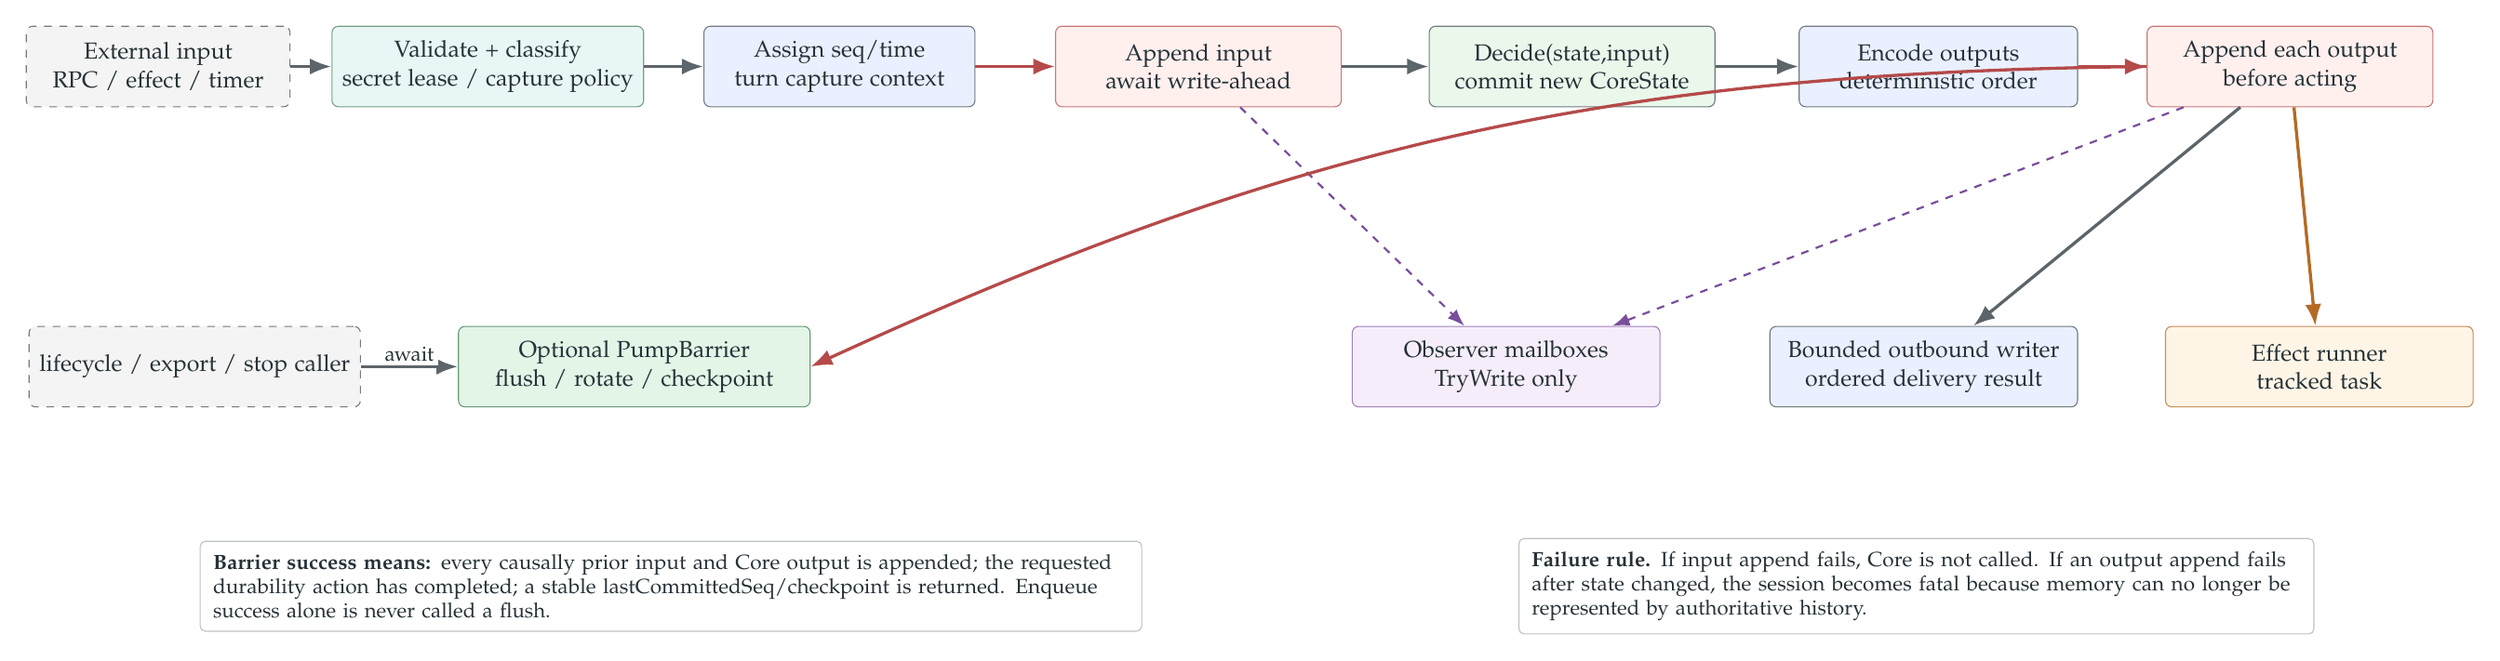
\begin{tikzpicture}[x=1cm,y=1cm]
  \node[extbox,minimum width=36mm] (input) at (1.5,8.0) {External input\\RPC / effect / timer};
  \node[policybox,minimum width=39mm] (validate) at (6.0,8.0) {Validate + classify\\secret lease / capture policy};
  \node[box,minimum width=37mm] (seq) at (10.8,8.0) {Assign seq/time\\turn capture context};
  \node[journalbox,minimum width=39mm] (jin) at (15.7,8.0) {Append input\\await write-ahead};
  \node[corebox,minimum width=39mm] (decide) at (20.8,8.0) {Decide(state,input)\\commit new CoreState};
  \node[box,minimum width=38mm] (encode) at (25.8,8.0) {Encode outputs\\deterministic order};
  \node[journalbox,minimum width=39mm] (jout) at (30.6,8.0) {Append each output\\before acting};
  \draw[arrow] (input) -- (validate); \draw[arrow] (validate) -- (seq);
  \draw[write] (seq) -- (jin); \draw[arrow] (jin) -- (decide);
  \draw[arrow] (decide) -- (encode); \draw[write] (encode) -- (jout);

  \node[box,minimum width=42mm] (rpc) at (25.6,3.9) {Bounded outbound writer\\ordered delivery result};
  \node[edgebox,minimum width=42mm] (effect) at (31.0,3.9) {Effect runner\\tracked task};
  \node[obsbox,minimum width=42mm] (obs) at (19.9,3.9) {Observer mailboxes\\TryWrite only};
  \draw[arrow] (jout) -- (rpc);
  \draw[effect] (jout) -- (effect);
  \draw[async] (jin) -- (obs);
  \draw[async] (jout) -- (obs);

  \node[goodbox,minimum width=48mm] (barrier) at (8.0,3.9) {Optional PumpBarrier\\flush / rotate / checkpoint};
  \draw[write] (jout.west) to[bend right=12] (barrier.east);
  \node[extbox,minimum width=42mm] (caller) at (2.0,3.9) {lifecycle / export / stop caller};
  \draw[arrow] (caller) -- node[label,above]{await} (barrier);

  \node[note,text width=125mm] at (8.5,0.9) {
    \textbf{Barrier success means:} every causally prior input and Core output is appended;
    the requested durability action has completed; a stable lastCommittedSeq/checkpoint is
    returned. Enqueue success alone is never called a flush.
  };
  \node[note,text width=105mm] at (25.5,0.9) {
    \textbf{Failure rule.} If input append fails, Core is not called. If an output append fails
    after state changed, the session becomes fatal because memory can no longer be represented
    by authoritative history.
  };
\end{tikzpicture}\end{adjustbox}
\clearpage

% -----------------------------------------------------------------------------
\pagehead{4. Fatal containment and pending-request drain}{A failed STS2 becomes unavailable; it does not become a black hole and does not kill legacy.}
\begin{adjustbox}{max width=0.98\linewidth,max totalheight=0.78\textheight,center}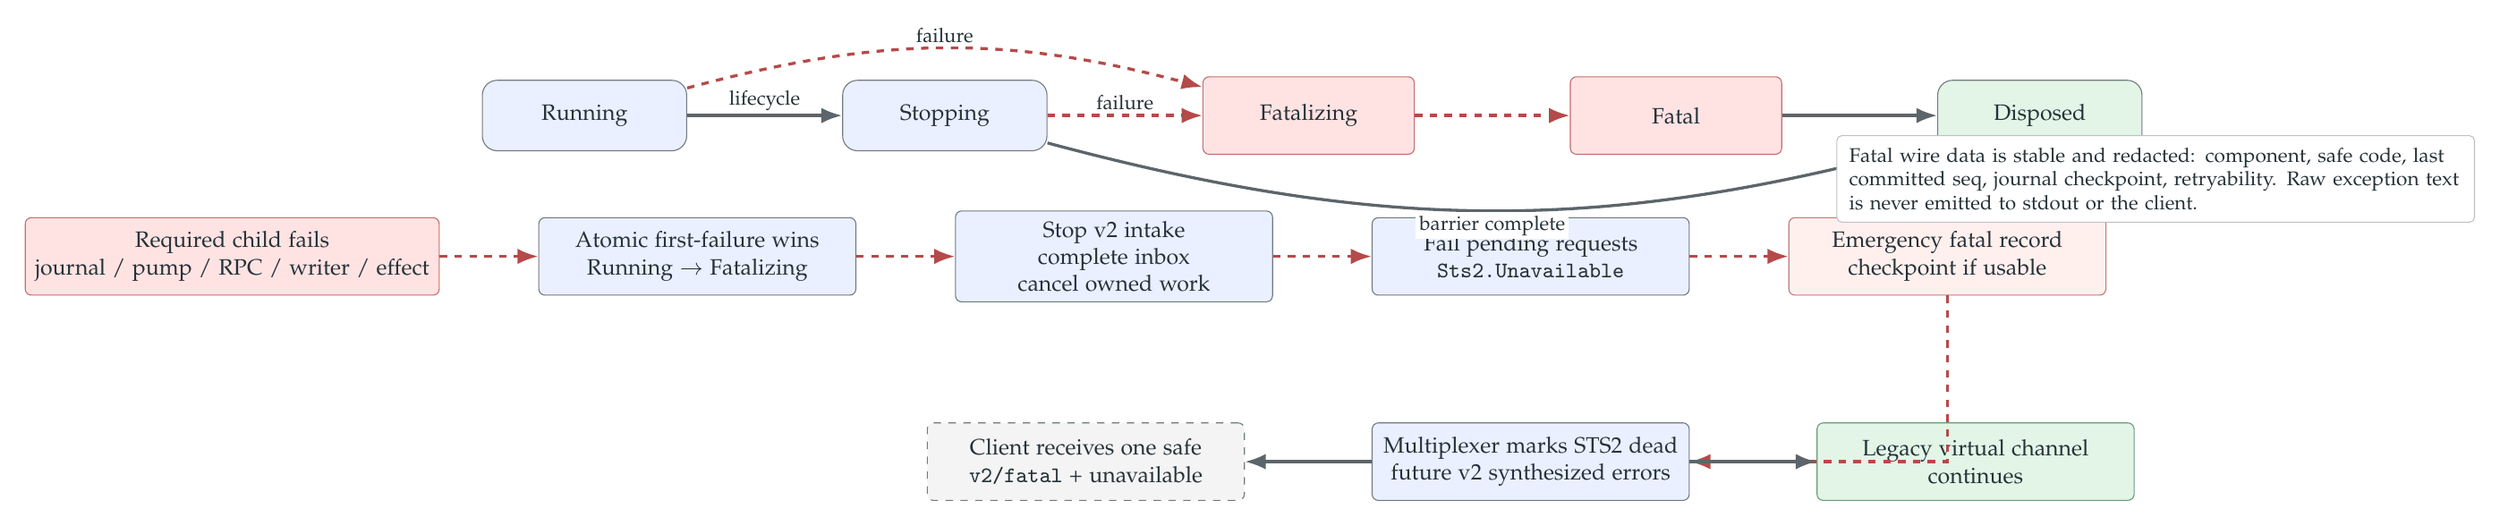
\begin{tikzpicture}[node distance=10mm and 14mm]
  \node[riskbox,minimum width=45mm] (fail) {Required child fails\\journal / pump / RPC / writer / effect};
  \node[box,right=of fail,minimum width=45mm] (cas) {Atomic first-failure wins\\Running $\rightarrow$ Fatalizing};
  \node[box,right=of cas,minimum width=45mm] (stop) {Stop v2 intake\\complete inbox\\cancel owned work};
  \node[box,right=of stop,minimum width=45mm] (pending) {Fail pending requests\\\code{Sts2.Unavailable}};
  \node[journalbox,right=of pending,minimum width=45mm] (emerg) {Emergency fatal record\\checkpoint if usable};
  \draw[fail] (fail) -- (cas); \draw[fail] (cas) -- (stop);
  \draw[fail] (stop) -- (pending); \draw[fail] (pending) -- (emerg);

  \node[box,below=18mm of pending,minimum width=45mm] (mux) {Multiplexer marks STS2 dead\\future v2 synthesized errors};
  \node[extbox,left=18mm of mux,minimum width=45mm] (client) {Client receives one safe\\\code{v2/fatal} + unavailable};
  \node[goodbox,right=18mm of mux,minimum width=45mm] (legacy) {Legacy virtual channel\\continues};
  \draw[fail] (emerg) |- (mux);
  \draw[arrow] (mux) -- (client);
  \draw[arrow] (mux) -- (legacy);

  \node[state] (running) at (5.0,2.0) {Running};
  \node[state,right=22mm of running] (stopping) {Stopping};
  \node[riskbox,right=22mm of stopping,minimum width=30mm] (fatalizing) {Fatalizing};
  \node[riskbox,right=22mm of fatalizing,minimum width=30mm] (fatal) {Fatal};
  \node[term,right=22mm of fatal] (disposed) {Disposed};
  \draw[arrow] (running) -- node[label,above]{lifecycle} (stopping);
  \draw[fail] (running) to[bend left=15] node[label,above]{failure} (fatalizing);
  \draw[fail] (stopping) -- node[label,above]{failure} (fatalizing);
  \draw[fail] (fatalizing) -- (fatal);
  \draw[arrow] (stopping) to[bend right=15] node[label,below]{barrier complete} (disposed);
  \draw[arrow] (fatal) -- (disposed);

  \node[note,text width=87mm] at (27.3,1.1) {
    Fatal wire data is stable and redacted: component, safe code, last committed seq, journal
    checkpoint, retryability. Raw exception text is never emitted to stdout or the client.
  };
\end{tikzpicture}\end{adjustbox}
\clearpage

% -----------------------------------------------------------------------------
\pagehead{5. Connection and query lifecycle}{Recommended target states make close, dispose, timeout, and waiter ownership explicit.}
\begin{adjustbox}{max width=0.98\linewidth,max totalheight=0.78\textheight,center}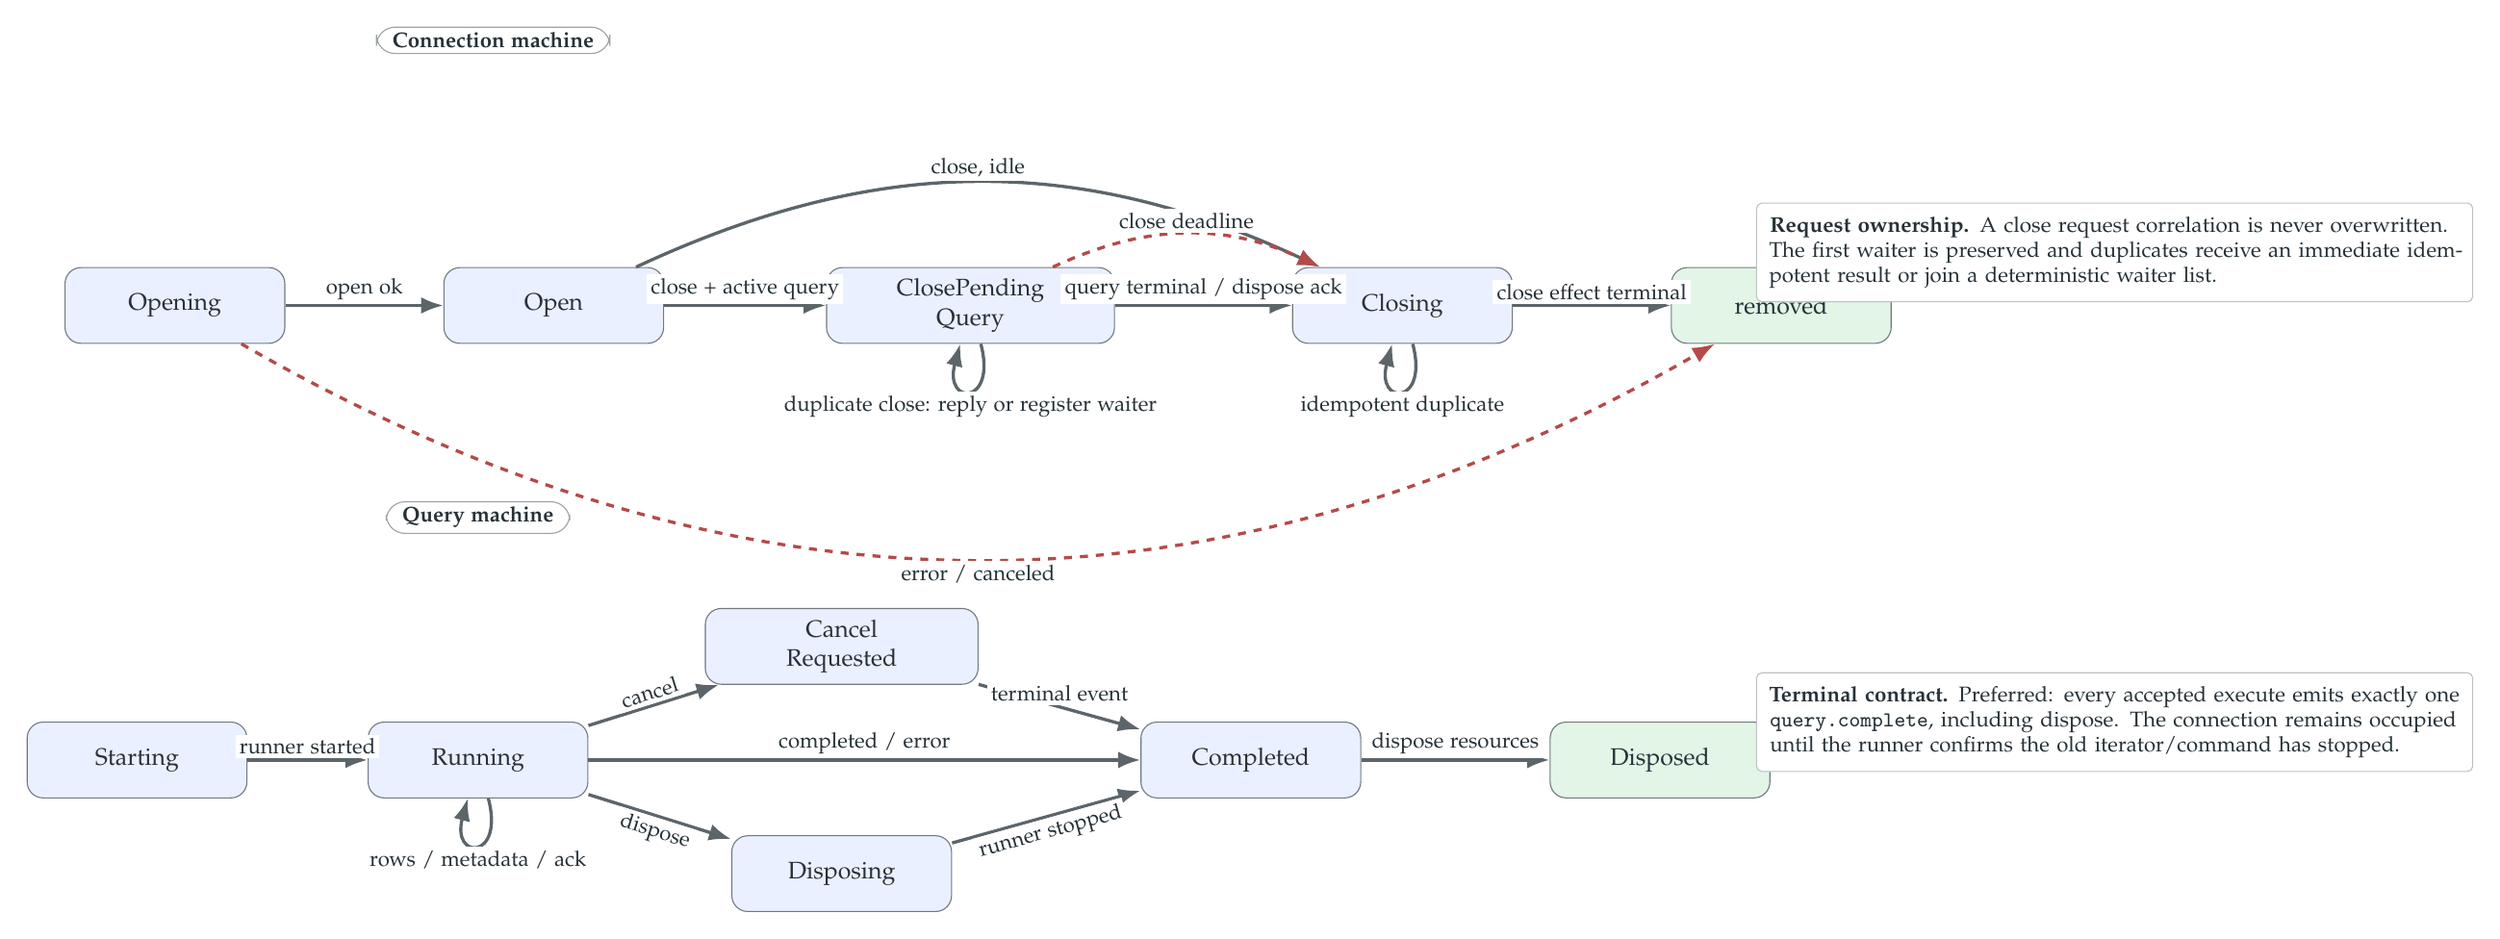
\begin{tikzpicture}[x=1cm,y=1cm]
  % Connection
  \node[pill] at (6.2,13.0) {Connection machine};
  \node[state] (co) at (2.0,9.5) {Opening};
  \node[state] (cop) at (7.0,9.5) {Open};
  \node[state,minimum width=38mm] (cp) at (12.5,9.5) {ClosePending\\Query};
  \node[state] (cc) at (18.2,9.5) {Closing};
  \node[term] (cx) at (23.2,9.5) {removed};
  \draw[arrow] (co) -- node[label,above]{open ok} (cop);
  \draw[fail] (co) to[bend right=30] node[label,below]{error / canceled} (cx);
  \draw[arrow] (cop) -- node[label,above]{close + active query} (cp);
  \draw[arrow] (cop) to[bend left=25] node[label,above]{close, idle} (cc);
  \draw[arrow] (cp) -- node[label,above]{query terminal / dispose ack} (cc);
  \draw[fail] (cp) to[bend left=25] node[label,above]{close deadline} (cc);
  \draw[arrow] (cc) -- node[label,above]{close effect terminal} (cx);
  \draw[arrow] (cp) to[loop below] node[label,below]{duplicate close: reply or register waiter} (cp);
  \draw[arrow] (cc) to[loop below] node[label,below]{idempotent duplicate} (cc);

  % Query
  \node[pill] at (6.0,6.7) {Query machine};
  \node[state] (qs) at (1.5,3.5) {Starting};
  \node[state] (qr) at (6.0,3.5) {Running};
  \node[state,minimum width=36mm] (qc) at (10.8,5.0) {Cancel\\Requested};
  \node[state] (qd) at (10.8,2.0) {Disposing};
  \node[state] (qdone) at (16.2,3.5) {Completed};
  \node[term] (qdisp) at (21.6,3.5) {Disposed};
  \draw[arrow] (qs) -- node[label,above]{runner started} (qr);
  \draw[arrow] (qr) -- node[label,above,sloped]{cancel} (qc);
  \draw[arrow] (qr) -- node[label,below,sloped]{dispose} (qd);
  \draw[arrow] (qr) -- node[label,above]{completed / error} (qdone);
  \draw[arrow] (qc) -- node[label,above]{terminal event} (qdone);
  \draw[arrow] (qd) -- node[label,below,sloped]{runner stopped} (qdone);
  \draw[arrow] (qdone) -- node[label,above]{dispose resources} (qdisp);
  \draw[arrow] (qr) to[loop below] node[label,below]{rows / metadata / ack} (qr);

  \node[note,text width=91mm] at (27.6,10.2) {
    \textbf{Request ownership.} A close request correlation is never overwritten. The first
    waiter is preserved and duplicates receive an immediate idempotent result or join a
    deterministic waiter list.
  };
  \node[note,text width=91mm] at (27.6,4.0) {
    \textbf{Terminal contract.} Preferred: every accepted execute emits exactly one
    \code{query.complete}, including dispose. The connection remains occupied until the
    runner confirms the old iterator/command has stopped.
  };
\end{tikzpicture}\end{adjustbox}
\clearpage

% -----------------------------------------------------------------------------
\pagehead{6. Backpressure at the real driver edge}{Credit is permission to request a page, not merely permission to send a notification.}
\begin{adjustbox}{max width=0.98\linewidth,max totalheight=0.78\textheight,center}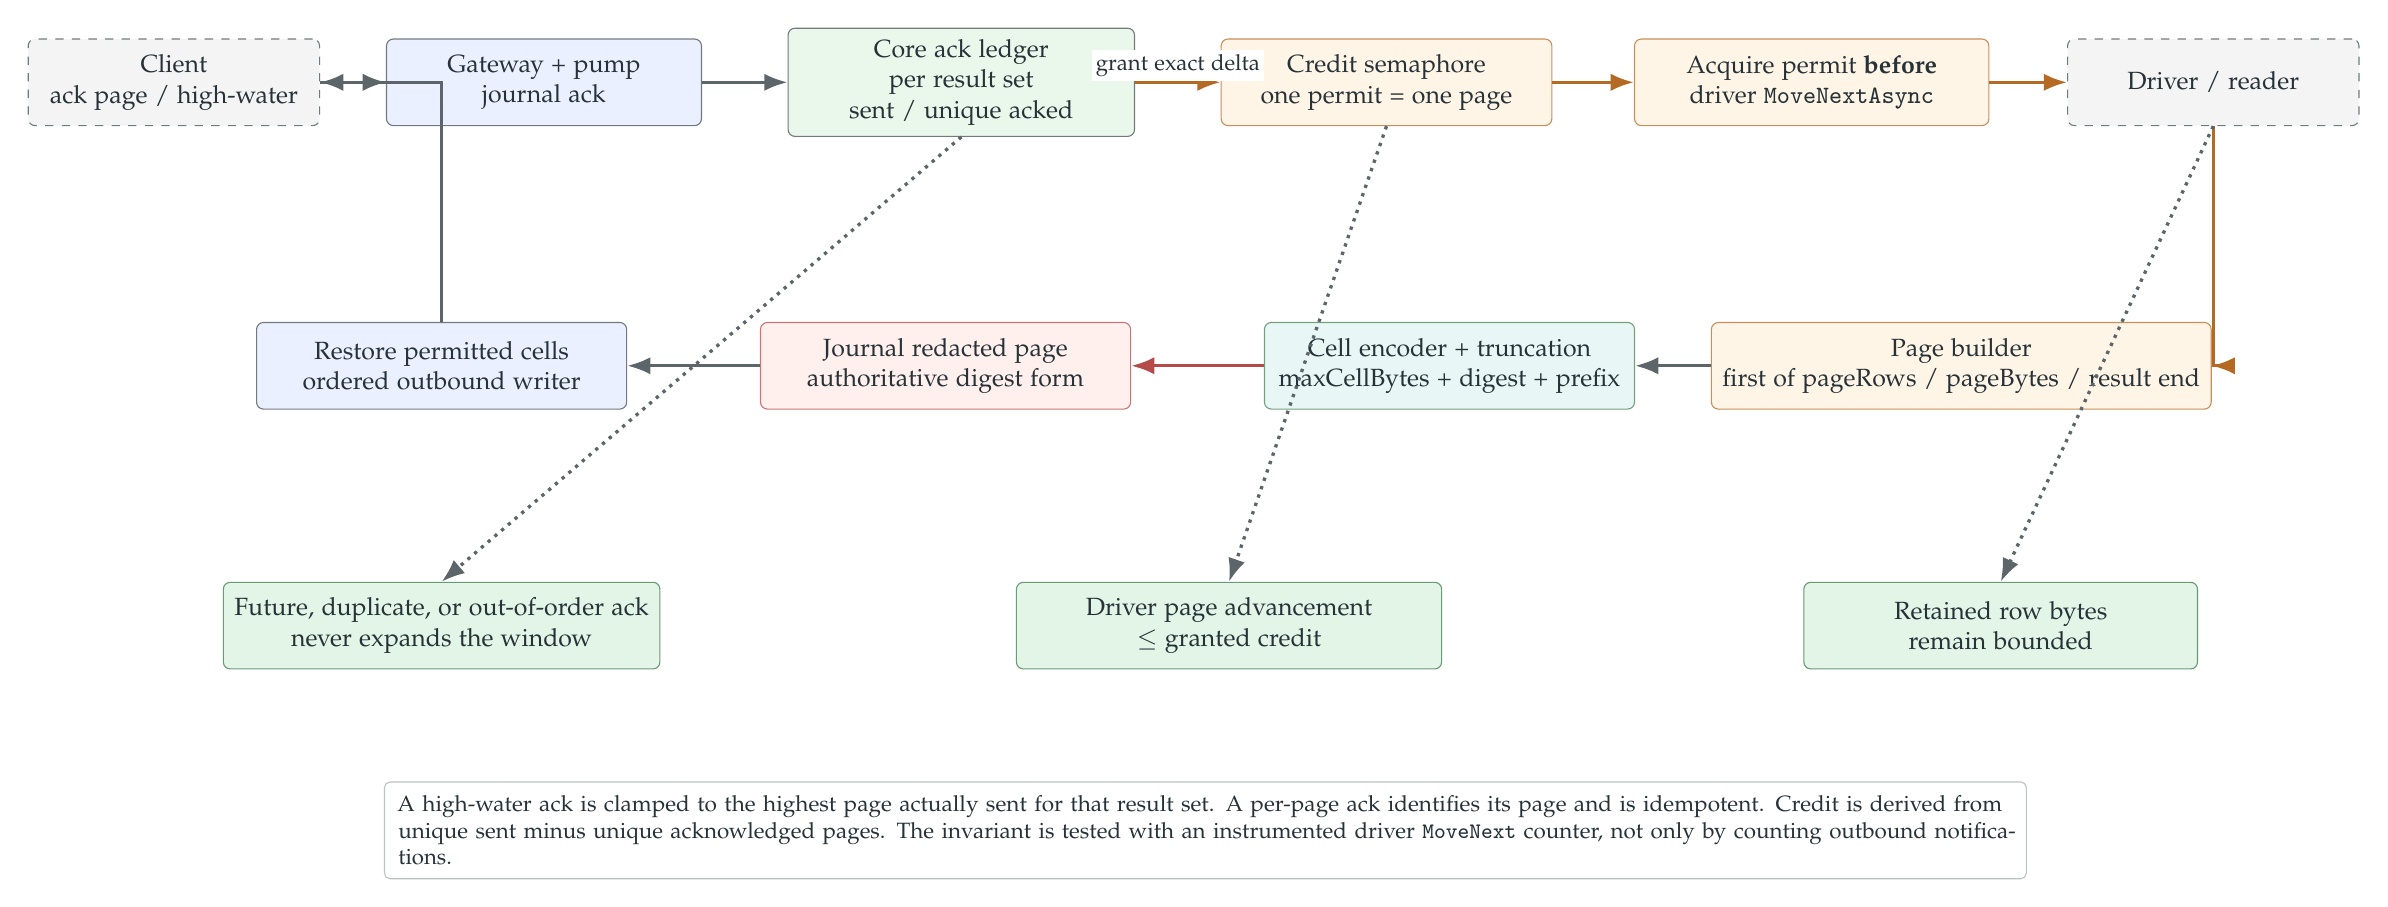
\begin{tikzpicture}[x=1cm,y=1cm]
  \node[extbox,minimum width=37mm] (client) at (1.6,10.2) {Client\\ack page / high-water};
  \node[box,minimum width=40mm] (gateway) at (6.3,10.2) {Gateway + pump\\journal ack};
  \node[corebox,minimum width=44mm] (ledger) at (11.6,10.2) {Core ack ledger\\per result set\\sent / unique acked};
  \node[edgebox,minimum width=42mm] (permit) at (17.0,10.2) {Credit semaphore\\one permit = one page};
  \node[edgebox,minimum width=45mm] (move) at (22.4,10.2) {Acquire permit \textbf{before}\\driver \code{MoveNextAsync}};
  \node[extbox,minimum width=37mm] (db) at (27.5,10.2) {Driver / reader};
  \draw[arrow] (client) -- (gateway);
  \draw[arrow] (gateway) -- (ledger);
  \draw[effect] (ledger) -- node[label,above]{grant exact delta} (permit);
  \draw[effect] (permit) -- (move);
  \draw[effect] (move) -- (db);

  \node[edgebox,minimum width=49mm] (builder) at (24.3,6.6) {Page builder\\first of pageRows / pageBytes / result end};
  \node[policybox,minimum width=47mm] (cell) at (17.8,6.6) {Cell encoder + truncation\\maxCellBytes + digest + prefix};
  \node[journalbox,minimum width=47mm] (journal) at (11.4,6.6) {Journal redacted page\\authoritative digest form};
  \node[box,minimum width=47mm] (wire) at (5.0,6.6) {Restore permitted cells\\ordered outbound writer};
  \draw[effect] (db) |- (builder);
  \draw[arrow] (builder) -- (cell);
  \draw[write] (cell) -- (journal);
  \draw[arrow] (journal) -- (wire);
  \draw[arrow] (wire) |- (client);

  \node[goodbox,minimum width=54mm] (inv1) at (5.0,3.3) {Future, duplicate, or out-of-order ack\\never expands the window};
  \node[goodbox,minimum width=54mm] (inv2) at (15.0,3.3) {Driver page advancement\\$\le$ granted credit};
  \node[goodbox,minimum width=50mm] (inv3) at (24.8,3.3) {Retained row bytes\\remain bounded};
  \draw[arrow,dotted] (ledger.south) -- (inv1.north);
  \draw[arrow,dotted] (permit.south) -- (inv2.north);
  \draw[arrow,dotted] (db.south) -- (inv3.north);

  \node[note,text width=205mm] at (14.7,0.7) {
    A high-water ack is clamped to the highest page actually sent for that result set. A
    per-page ack identifies its page and is idempotent. Credit is derived from unique sent
    minus unique acknowledged pages. The invariant is tested with an instrumented driver
    \code{MoveNext} counter, not only by counting outbound notifications.
  };
\end{tikzpicture}\end{adjustbox}
\clearpage

% -----------------------------------------------------------------------------
\pagehead{7. Run-scoped journal and strict replay}{Time travel may be partial; verification must prove a complete, internally valid run.}
\begin{adjustbox}{max width=0.98\linewidth,max totalheight=0.78\textheight,center}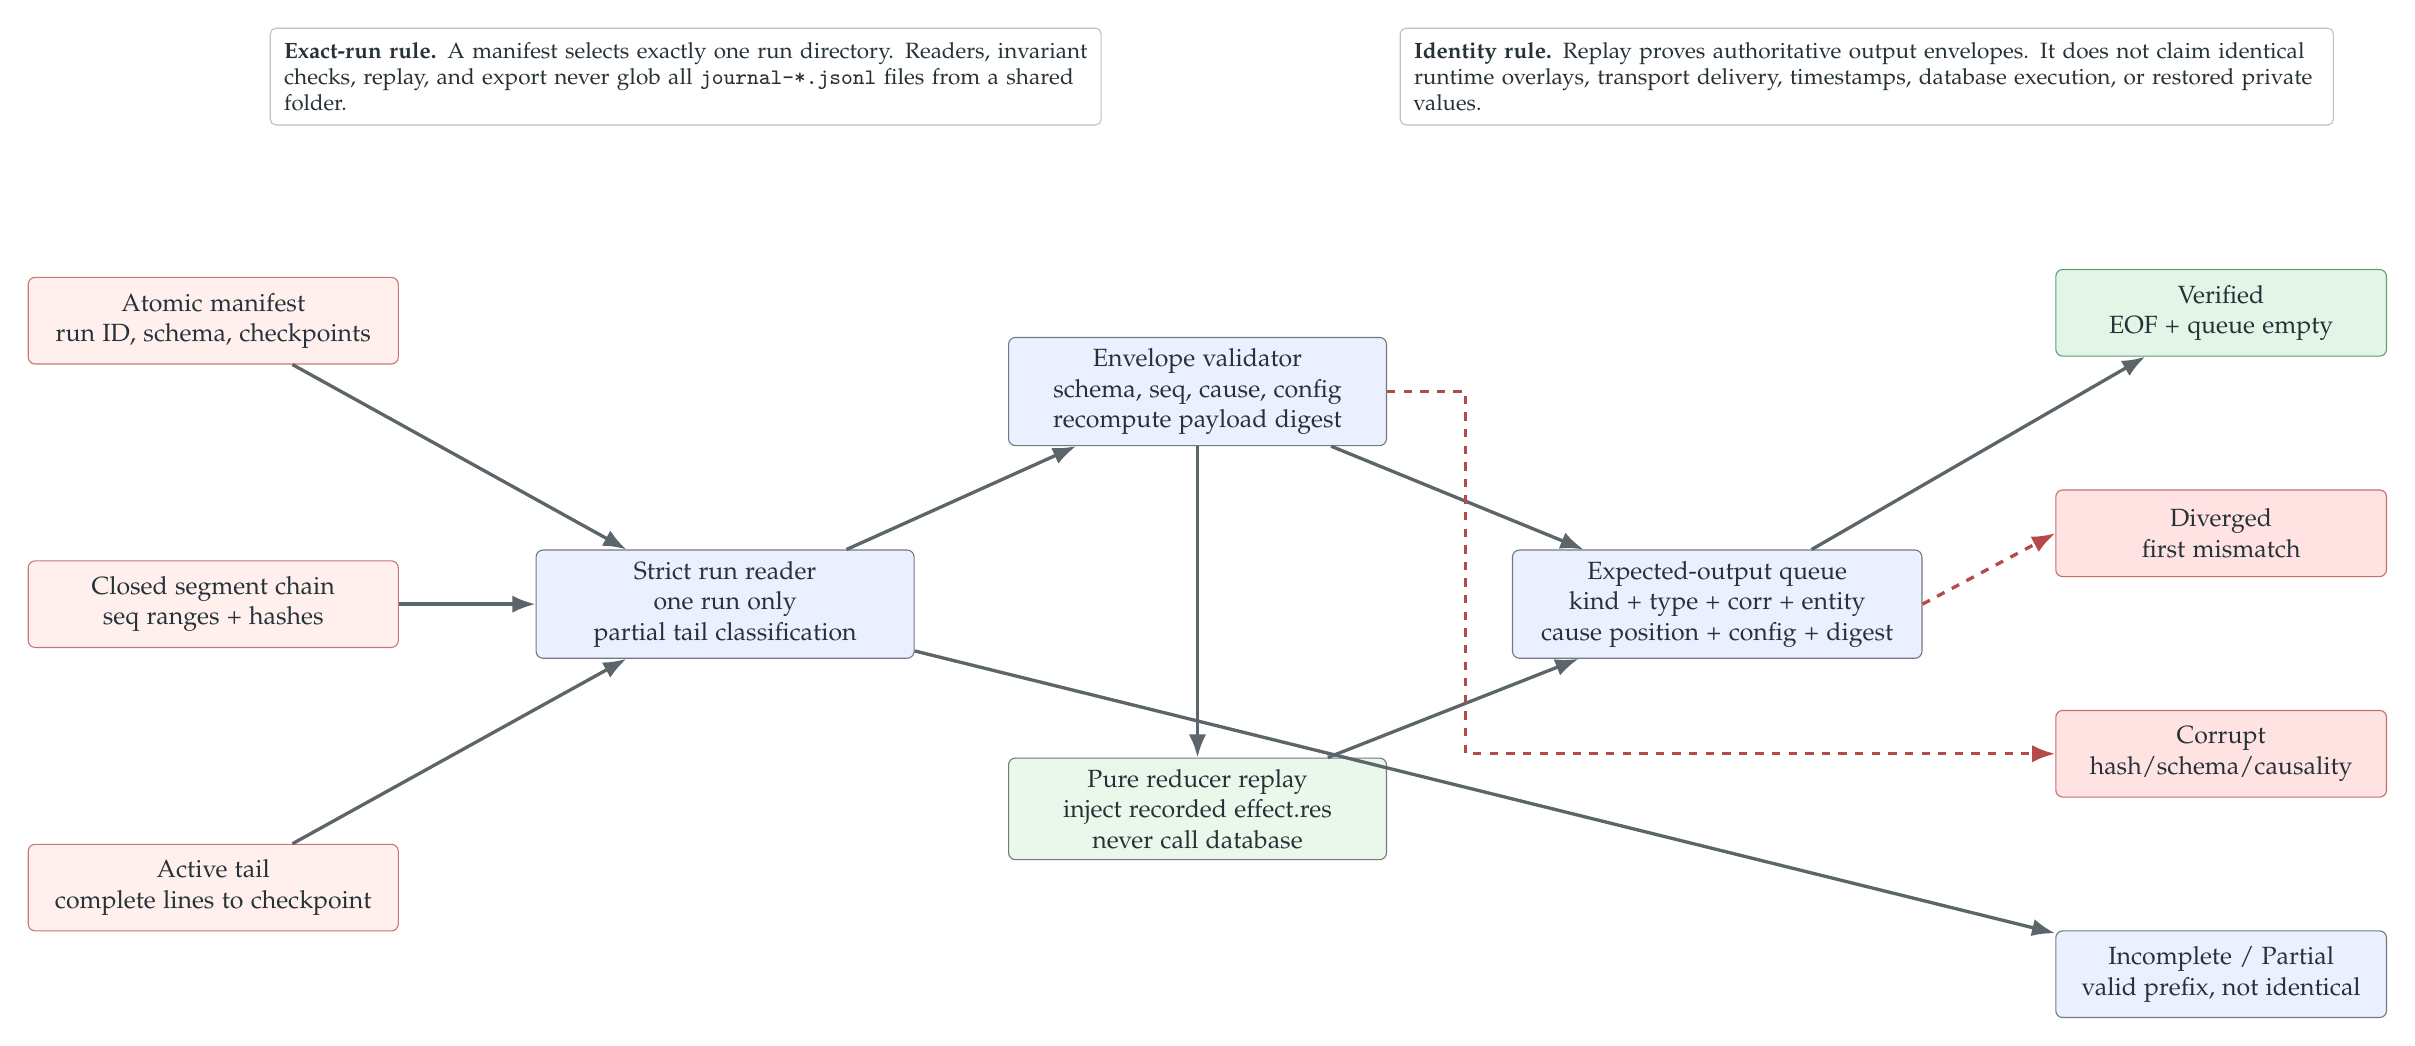
\begin{tikzpicture}[x=1cm,y=1cm]
  \node[journalbox,minimum width=47mm] (manifest) at (2.5,9.4) {Atomic manifest\\run ID, schema, checkpoints};
  \node[journalbox,minimum width=47mm] (segments) at (2.5,5.8) {Closed segment chain\\seq ranges + hashes};
  \node[journalbox,minimum width=47mm] (active) at (2.5,2.2) {Active tail\\complete lines to checkpoint};
  \node[box,minimum width=48mm] (reader) at (9.0,5.8) {Strict run reader\\one run only\\partial tail classification};
  \draw[arrow] (manifest) -- (reader); \draw[arrow] (segments) -- (reader); \draw[arrow] (active) -- (reader);

  \node[box,minimum width=48mm] (validate) at (15.0,8.5) {Envelope validator\\schema, seq, cause, config\\recompute payload digest};
  \node[corebox,minimum width=48mm] (reducer) at (15.0,3.2) {Pure reducer replay\\inject recorded effect.res\\never call database};
  \draw[arrow] (reader) -- (validate);
  \draw[arrow] (validate) -- (reducer);

  \node[box,minimum width=52mm] (queue) at (21.6,5.8) {Expected-output queue\\kind + type + corr + entity\\cause position + config + digest};
  \draw[arrow] (reducer) -- (queue);
  \draw[arrow] (validate) -- (queue);

  \node[goodbox,minimum width=42mm] (verified) at (28.0,9.5) {Verified\\EOF + queue empty};
  \node[riskbox,minimum width=42mm] (div) at (28.0,6.7) {Diverged\\first mismatch};
  \node[riskbox,minimum width=42mm] (corrupt) at (28.0,3.9) {Corrupt\\hash/schema/causality};
  \node[box,minimum width=42mm] (partial) at (28.0,1.1) {Incomplete / Partial\\valid prefix, not identical};
  \draw[arrow] (queue) -- (verified);
  \draw[fail] (queue.east) -- (div.west);
  \draw[fail] (validate.east) -- ++(1.0,0) |- (corrupt.west);
  \draw[arrow] (reader) -- (partial);

  \node[note,text width=102mm] at (8.5,12.5) {
    \textbf{Exact-run rule.} A manifest selects exactly one run directory. Readers, invariant
    checks, replay, and export never glob all \code{journal-*.jsonl} files from a shared folder.
  };
  \node[note,text width=115mm] at (23.5,12.5) {
    \textbf{Identity rule.} Replay proves authoritative output envelopes. It does not claim
    identical runtime overlays, transport delivery, timestamps, database execution, or
    restored private values.
  };
\end{tikzpicture}\end{adjustbox}
\clearpage

% -----------------------------------------------------------------------------
\pagehead{8. Privacy by policy and scoped restoration}{Sensitive originals have short, owned lifetimes and never reach the authoritative journal by accident.}
\begin{adjustbox}{max width=0.98\linewidth,max totalheight=0.78\textheight,center}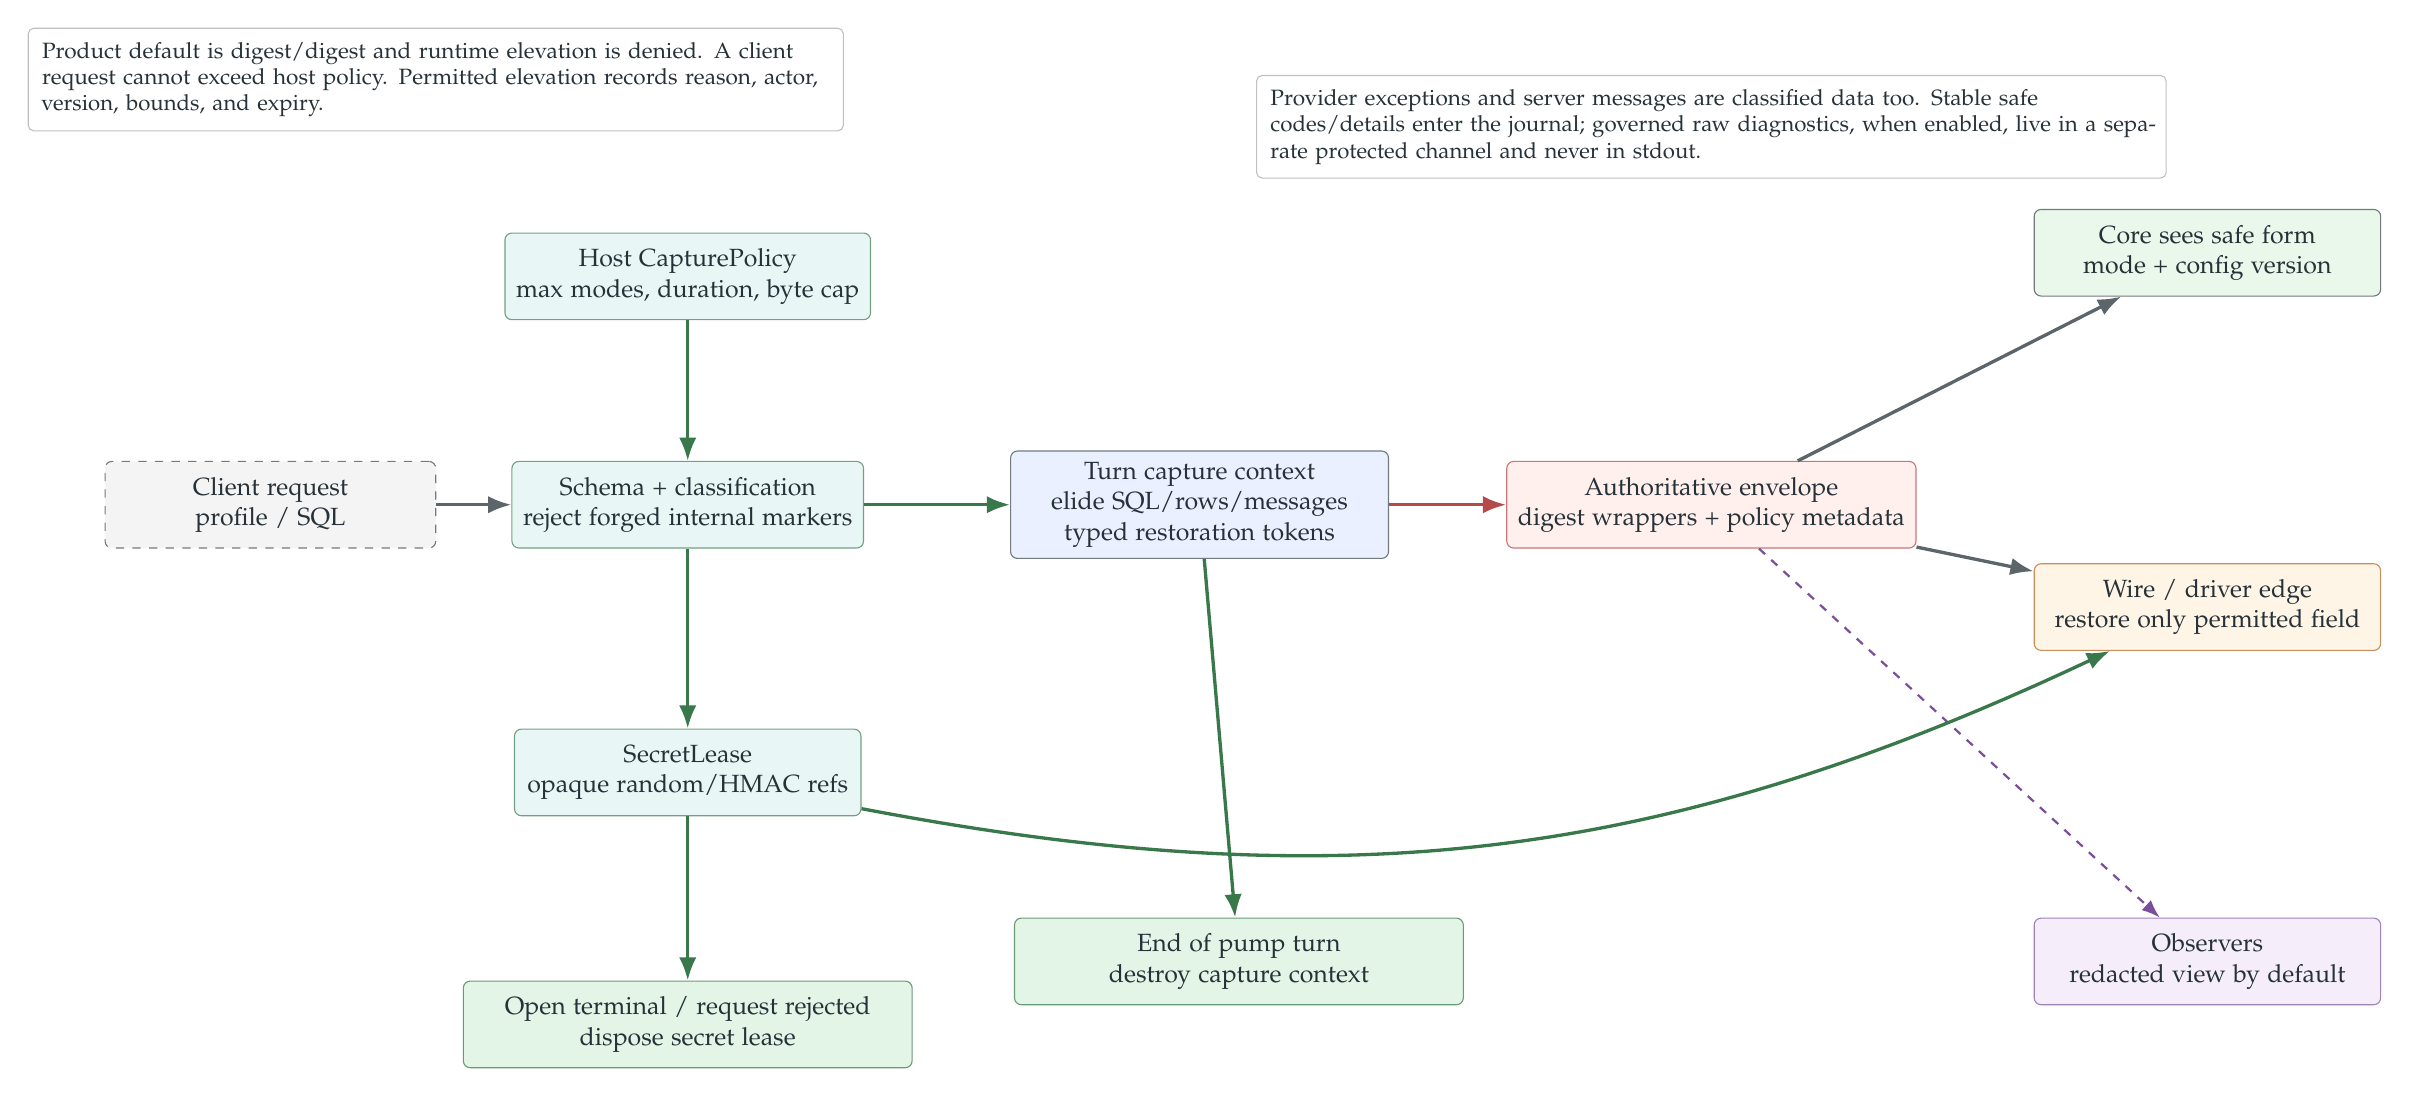
\begin{tikzpicture}[x=1cm,y=1cm]
  \node[extbox,minimum width=42mm] (req) at (1.7,8.0) {Client request\\profile / SQL};
  \node[policybox,minimum width=44mm] (policy) at (7.0,10.9) {Host CapturePolicy\\max modes, duration, byte cap};
  \node[policybox,minimum width=44mm] (validate) at (7.0,8.0) {Schema + classification\\reject forged internal markers};
  \node[policybox,minimum width=44mm] (secret) at (7.0,4.6) {SecretLease\\opaque random/HMAC refs};
  \node[box,minimum width=48mm] (turn) at (13.5,8.0) {Turn capture context\\elide SQL/rows/messages\\typed restoration tokens};
  \node[journalbox,minimum width=49mm] (journal) at (20.0,8.0) {Authoritative envelope\\digest wrappers + policy metadata};
  \node[corebox,minimum width=44mm] (core) at (26.3,11.2) {Core sees safe form\\mode + config version};
  \node[edgebox,minimum width=44mm] (edge) at (26.3,6.7) {Wire / driver edge\\restore only permitted field};
  \node[obsbox,minimum width=44mm] (obs) at (26.3,2.2) {Observers\\redacted view by default};
  \draw[arrow] (req) -- (validate);
  \draw[policyarr] (policy) -- (validate);
  \draw[policyarr] (validate) -- (secret);
  \draw[policyarr] (validate) -- (turn);
  \draw[write] (turn) -- (journal);
  \draw[arrow] (journal) -- (core);
  \draw[arrow] (journal) -- (edge);
  \draw[async] (journal) -- (obs);
  \draw[policyarr] (secret) to[bend right=18] (edge);

  \node[goodbox,minimum width=57mm] (destroy) at (14.0,2.2) {End of pump turn\\destroy capture context};
  \draw[policyarr] (turn) -- (destroy);
  \node[goodbox,minimum width=57mm] (remove) at (7.0,1.4) {Open terminal / request rejected\\dispose secret lease};
  \draw[policyarr] (secret) -- (remove);

  \node[note,text width=100mm] at (3.8,13.4) {
    Product default is digest/digest and runtime elevation is denied. A client request cannot
    exceed host policy. Permitted elevation records reason, actor, version, bounds, and expiry.
  };
  \node[note,text width=112mm] at (20.0,12.8) {
    Provider exceptions and server messages are classified data too. Stable safe codes/details
    enter the journal; governed raw diagnostics, when enabled, live in a separate protected
    channel and never in stdout.
  };
\end{tikzpicture}\end{adjustbox}
\clearpage

% -----------------------------------------------------------------------------
\pagehead{9. Observer isolation and exact viewer resynchronization}{The pump publishes references; observer code runs behind bounded mailboxes.}
\begin{adjustbox}{max width=0.98\linewidth,max totalheight=0.78\textheight,center}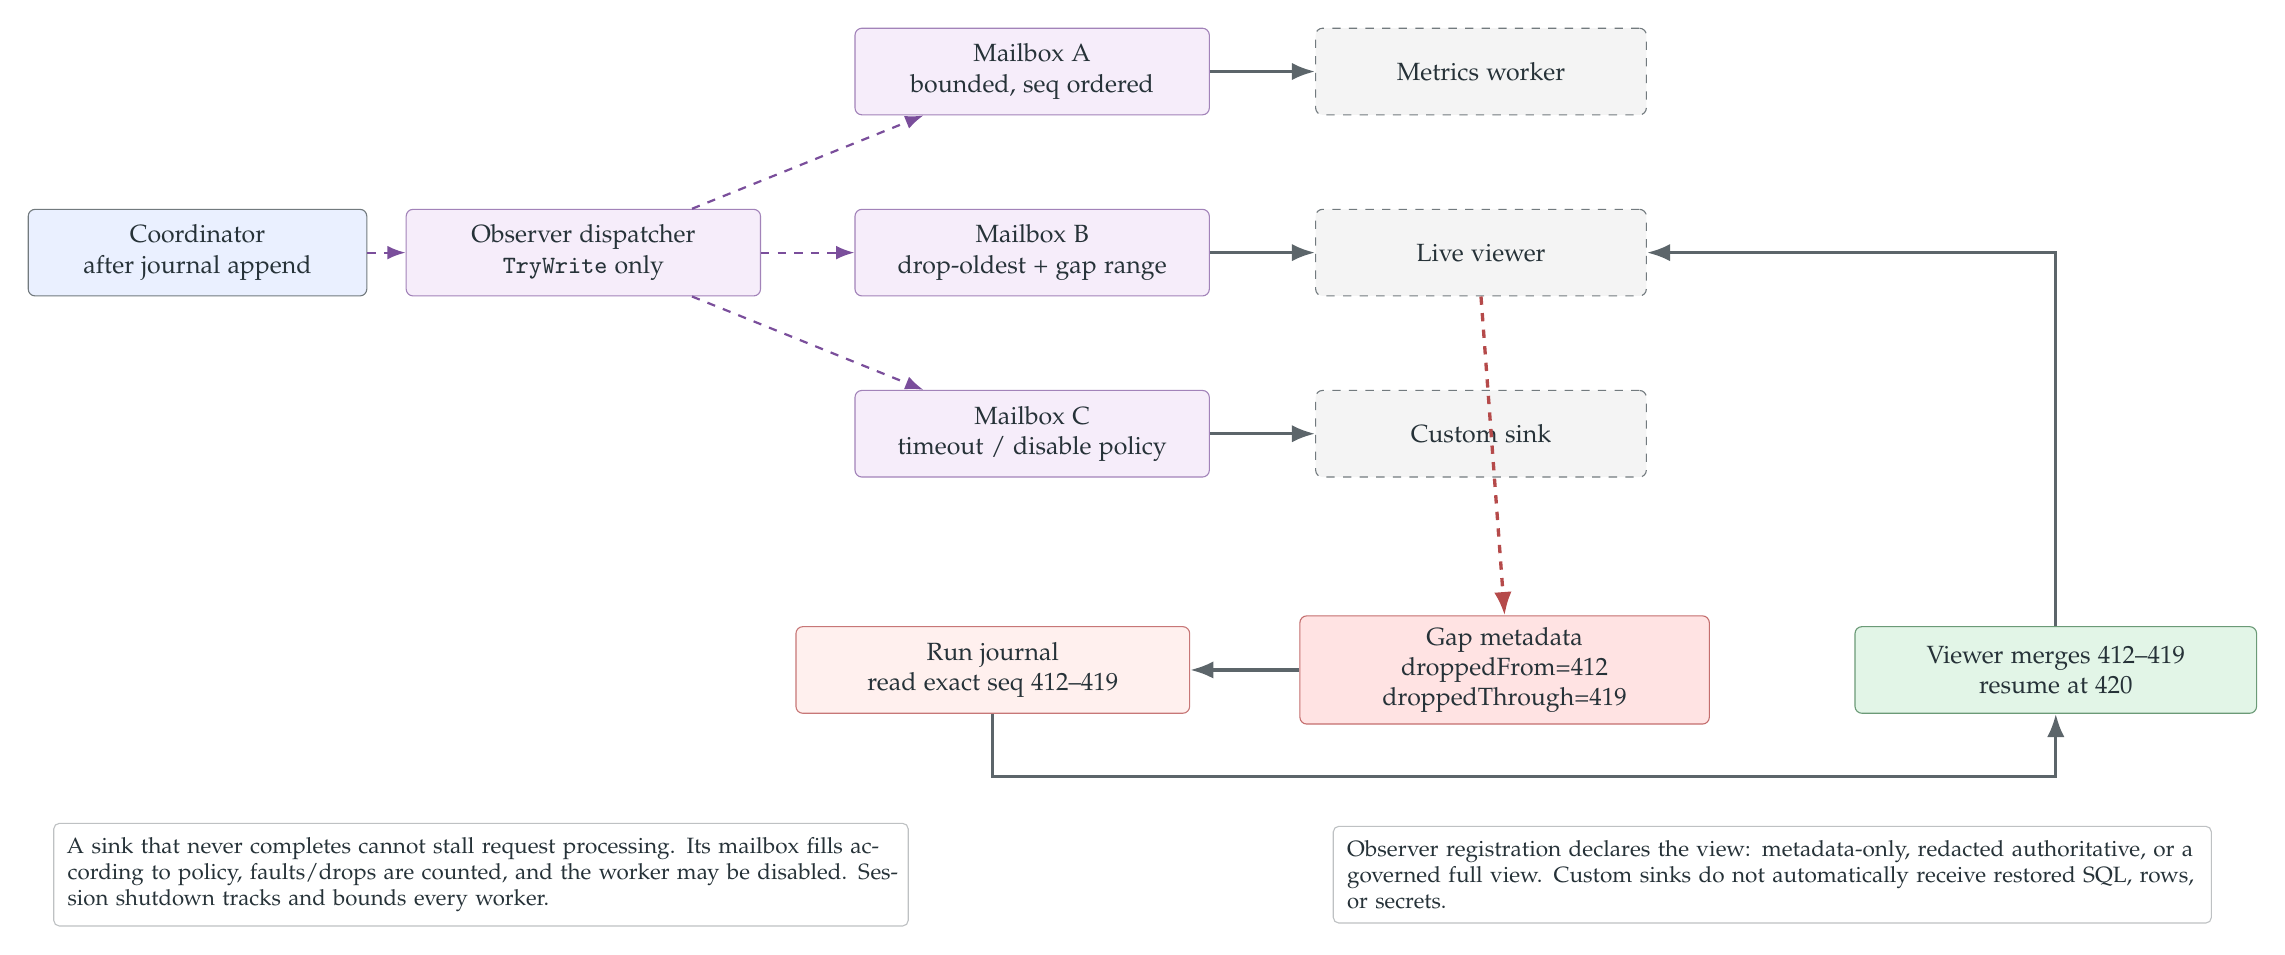
\begin{tikzpicture}[x=1cm,y=1cm]
  \node[box,minimum width=43mm] (pump) at (2.4,8.0) {Coordinator\\after journal append};
  \node[obsbox,minimum width=45mm] (dispatch) at (7.3,8.0) {Observer dispatcher\\\code{TryWrite} only};
  \draw[async] (pump) -- (dispatch);

  \node[obsbox,minimum width=45mm] (m1) at (13.0,10.3) {Mailbox A\\bounded, seq ordered};
  \node[obsbox,minimum width=45mm] (m2) at (13.0,8.0) {Mailbox B\\drop-oldest + gap range};
  \node[obsbox,minimum width=45mm] (m3) at (13.0,5.7) {Mailbox C\\timeout / disable policy};
  \draw[async] (dispatch) -- (m1); \draw[async] (dispatch) -- (m2); \draw[async] (dispatch) -- (m3);

  \node[extbox,minimum width=42mm] (metrics) at (18.7,10.3) {Metrics worker};
  \node[extbox,minimum width=42mm] (viewer) at (18.7,8.0) {Live viewer};
  \node[extbox,minimum width=42mm] (custom) at (18.7,5.7) {Custom sink};
  \draw[arrow] (m1) -- (metrics); \draw[arrow] (m2) -- (viewer); \draw[arrow] (m3) -- (custom);

  \node[journalbox,minimum width=50mm] (jr) at (12.5,2.7) {Run journal\\read exact seq 412--419};
  \node[riskbox,minimum width=52mm] (gap) at (19.0,2.7) {Gap metadata\\droppedFrom=412\\droppedThrough=419};
  \node[goodbox,minimum width=51mm] (resume) at (26.0,2.7) {Viewer merges 412--419\\resume at 420};
  \draw[fail] (viewer.south) -- (gap.north);
  \draw[arrow] (gap.west) -- (jr.east);
  \draw[arrow] (jr.south) -- ++(0,-0.8) -| (resume.south);
  \draw[arrow] (resume.north) |- (viewer.east);

  \node[note,text width=105mm] at (6.0,0.1) {
    A sink that never completes cannot stall request processing. Its mailbox fills according
    to policy, faults/drops are counted, and the worker may be disabled. Session shutdown
    tracks and bounds every worker.
  };
  \node[note,text width=108mm] at (22.4,0.1) {
    Observer registration declares the view: metadata-only, redacted authoritative, or a
    governed full view. Custom sinks do not automatically receive restored SQL, rows, or
    secrets.
  };
\end{tikzpicture}\end{adjustbox}
\clearpage

% -----------------------------------------------------------------------------
\pagehead{10. Coherent export and verification}{Export freezes an exact checkpoint, then copies and transforms outside the pump.}
\begin{adjustbox}{max width=0.98\linewidth,max totalheight=0.78\textheight,center}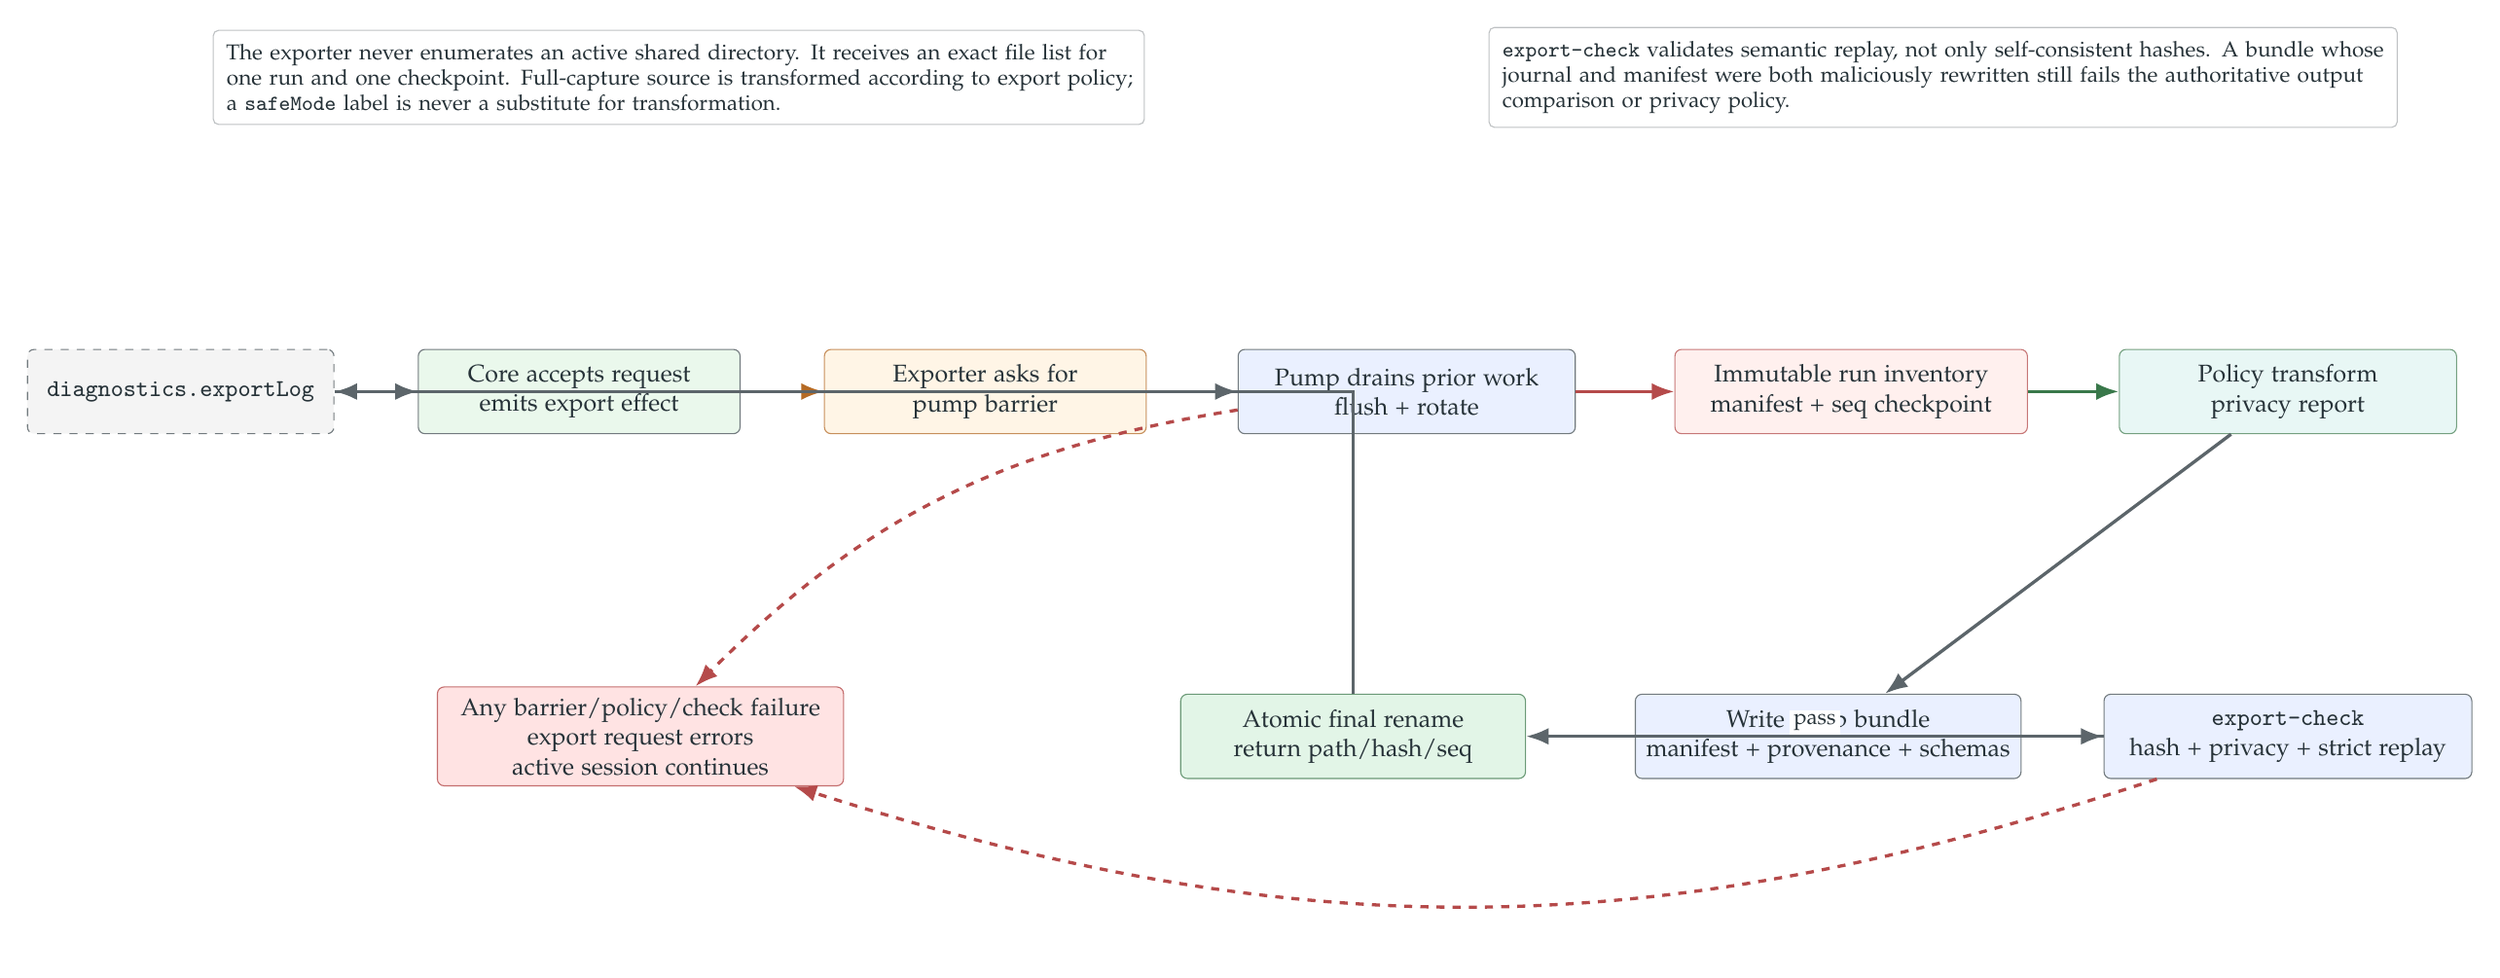
\begin{tikzpicture}[x=1cm,y=1cm]
  \node[extbox,minimum width=40mm] (client) at (1.5,7.5) {\code{diagnostics.exportLog}};
  \node[corebox,minimum width=42mm] (core) at (6.7,7.5) {Core accepts request\\emits export effect};
  \node[edgebox,minimum width=42mm] (effect) at (12.0,7.5) {Exporter asks for\\pump barrier};
  \node[box,minimum width=44mm] (barrier) at (17.5,7.5) {Pump drains prior work\\flush + rotate};
  \node[journalbox,minimum width=46mm] (inventory) at (23.3,7.5) {Immutable run inventory\\manifest + seq checkpoint};
  \node[policybox,minimum width=44mm] (transform) at (29.0,7.5) {Policy transform\\privacy report};
  \draw[arrow] (client) -- (core); \draw[effect] (core) -- (effect);
  \draw[arrow] (effect) -- (barrier); \draw[write] (barrier) -- (inventory);
  \draw[policyarr] (inventory) -- (transform);

  \node[box,minimum width=48mm] (zip) at (23.0,3.0) {Write temp bundle\\manifest + provenance + schemas};
  \node[box,minimum width=48mm] (check) at (29.0,3.0) {\code{export-check}\\hash + privacy + strict replay};
  \node[goodbox,minimum width=45mm] (rename) at (16.8,3.0) {Atomic final rename\\return path/hash/seq};
  \draw[arrow] (transform) -- (zip);
  \draw[arrow] (zip) -- (check);
  \draw[arrow] (check) -- node[label,above]{pass} (rename);
  \draw[arrow] (rename) |- (client);

  \node[riskbox,minimum width=53mm] (fail) at (7.5,3.0) {Any barrier/policy/check failure\\export request errors\\active session continues};
  \draw[fail] (barrier) to[bend right=18] (fail);
  \draw[fail] (check) to[bend left=18] (fail);

  \node[note,text width=118mm] at (8.0,11.6) {
    The exporter never enumerates an active shared directory. It receives an exact file list
    for one run and one checkpoint. Full-capture source is transformed according to export
    policy; a \code{safeMode} label is never a substitute for transformation.
  };
  \node[note,text width=115mm] at (24.5,11.6) {
    \code{export-check} validates semantic replay, not only self-consistent hashes. A bundle
    whose journal and manifest were both maliciously rewritten still fails the authoritative
    output comparison or privacy policy.
  };
\end{tikzpicture}\end{adjustbox}
\clearpage

% -----------------------------------------------------------------------------
\pagehead{11. Release evidence and adoption ladder}{The exact merge candidate, not mutable prose, earns the preview tag.}
\begin{adjustbox}{max width=0.98\linewidth,max totalheight=0.78\textheight,center}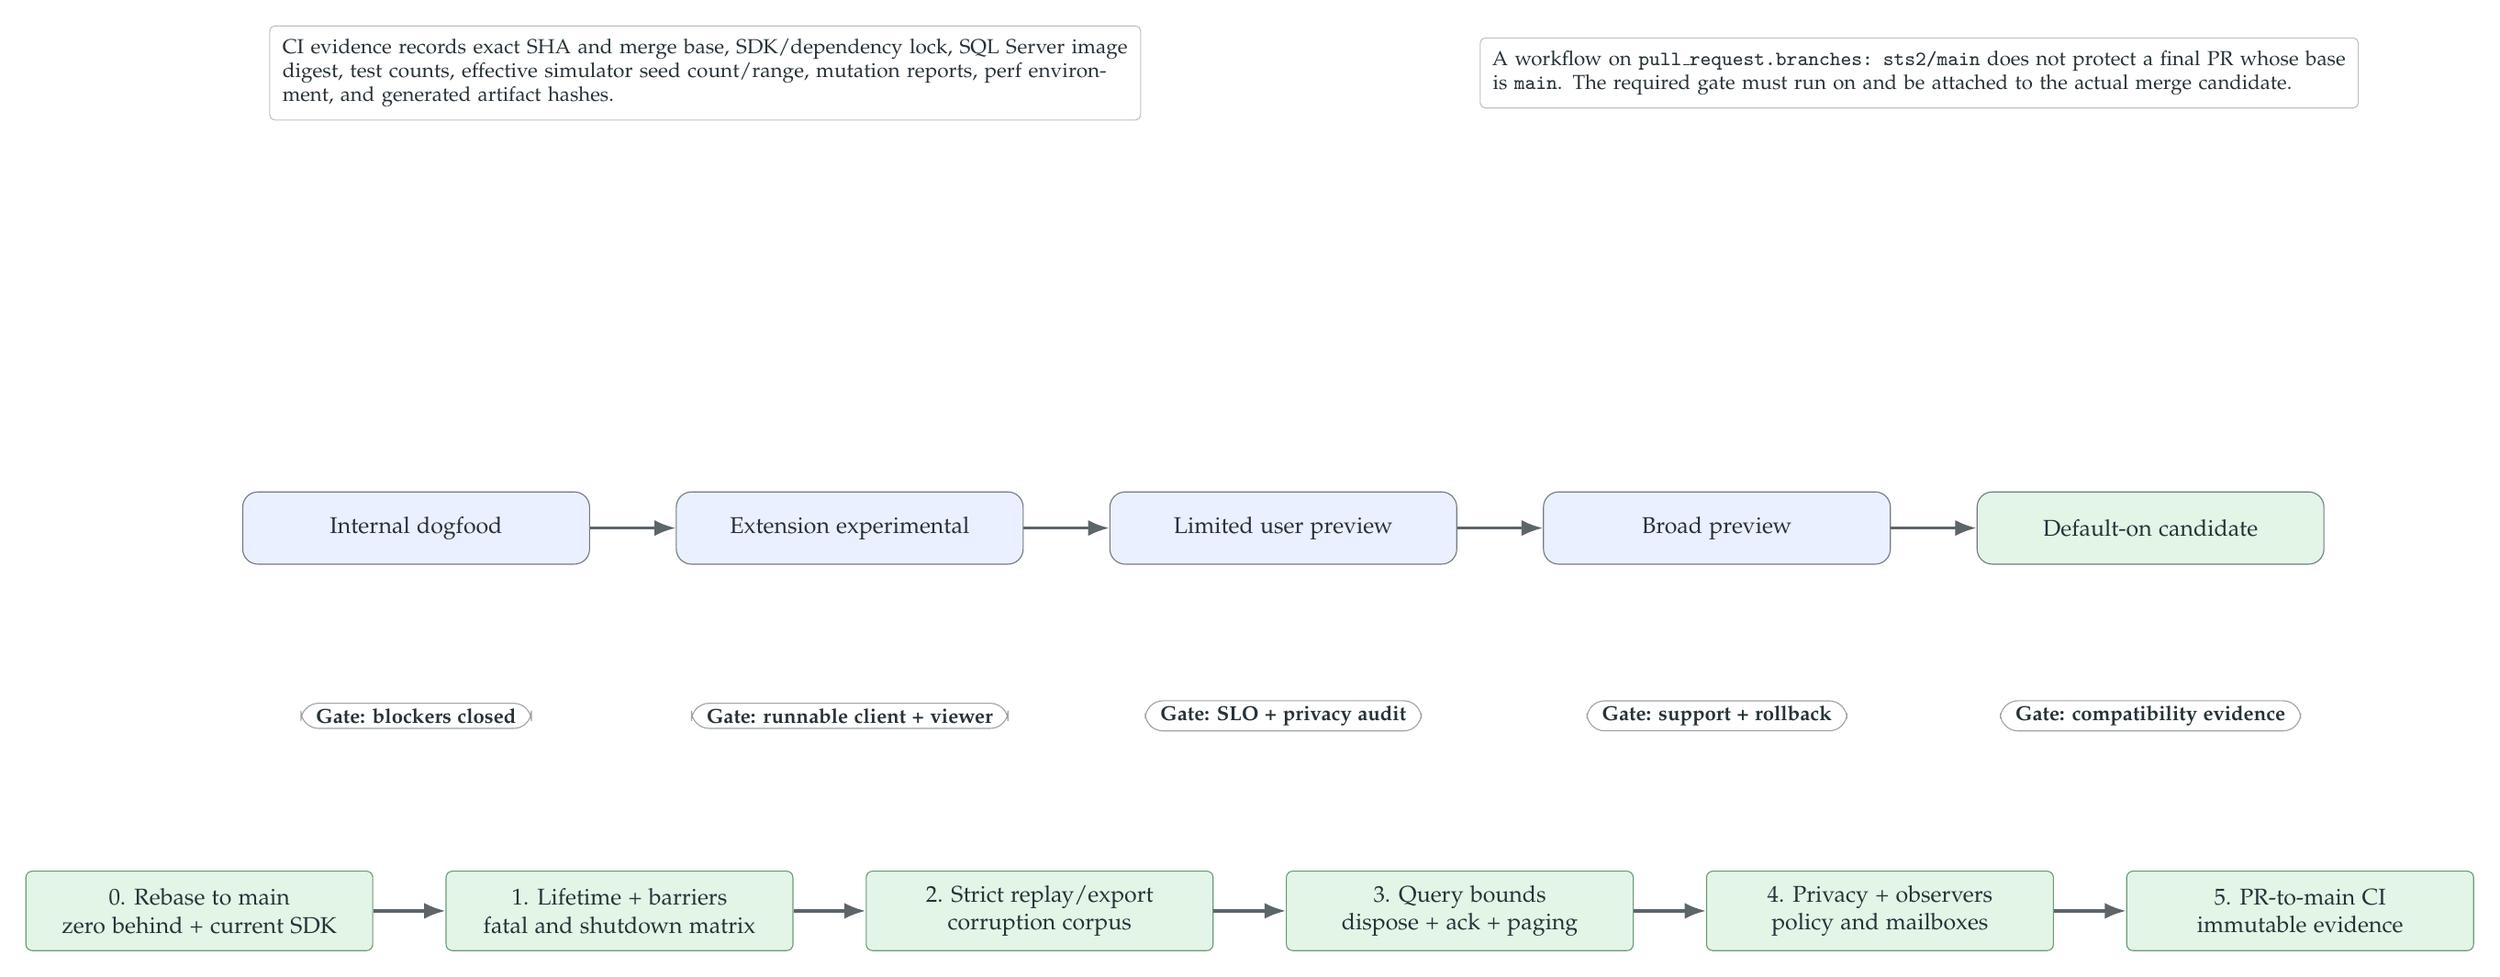
\begin{tikzpicture}[node distance=8mm and 10mm]
  \node[goodbox,minimum width=48mm] (base) {0. Rebase to main\\zero behind + current SDK};
  \node[goodbox,right=of base,minimum width=48mm] (life) {1. Lifetime + barriers\\fatal and shutdown matrix};
  \node[goodbox,right=of life,minimum width=48mm] (replay) {2. Strict replay/export\\corruption corpus};
  \node[goodbox,right=of replay,minimum width=48mm] (query) {3. Query bounds\\dispose + ack + paging};
  \node[goodbox,right=of query,minimum width=48mm] (privacy) {4. Privacy + observers\\policy and mailboxes};
  \node[goodbox,right=of privacy,minimum width=48mm] (ci) {5. PR-to-main CI\\immutable evidence};
  \draw[arrow] (base) -- (life); \draw[arrow] (life) -- (replay); \draw[arrow] (replay) -- (query);
  \draw[arrow] (query) -- (privacy); \draw[arrow] (privacy) -- (ci);

  \node[state,minimum width=48mm] (dog) at (3.0,5.3) {Internal dogfood};
  \node[state,minimum width=48mm] (exp) at (9.0,5.3) {Extension experimental};
  \node[state,minimum width=48mm] (limited) at (15.0,5.3) {Limited user preview};
  \node[state,minimum width=48mm] (broad) at (21.0,5.3) {Broad preview};
  \node[term,minimum width=48mm] (default) at (27.0,5.3) {Default-on candidate};
  \draw[arrow] (dog) -- (exp); \draw[arrow] (exp) -- (limited);
  \draw[arrow] (limited) -- (broad); \draw[arrow] (broad) -- (default);

  \node[pill] at (3.0,2.7) {Gate: blockers closed};
  \node[pill] at (9.0,2.7) {Gate: runnable client + viewer};
  \node[pill] at (15.0,2.7) {Gate: SLO + privacy audit};
  \node[pill] at (21.0,2.7) {Gate: support + rollback};
  \node[pill] at (27.0,2.7) {Gate: compatibility evidence};

  \node[note,text width=117mm] at (7.0,11.6) {
    CI evidence records exact SHA and merge base, SDK/dependency lock, SQL Server image digest,
    test counts, effective simulator seed count/range, mutation reports, perf environment, and
    generated artifact hashes.
  };
  \node[note,text width=118mm] at (23.8,11.6) {
    A workflow on \code{pull\_request.branches: sts2/main} does not protect a final PR whose
    base is \code{main}. The required gate must run on and be attached to the actual merge
    candidate.
  };
\end{tikzpicture}\end{adjustbox}

\vfill
{\small\color{muted}\legend}
\end{document}
